\documentclass[10pt, reqno]{amsart}
% \pdfoutput=1



% Packages to open
\usepackage{amsthm, amssymb, amsmath, enumerate, textcomp}
% \usepackage{fullpage}
\usepackage{verbatim}
\usepackage{graphicx, graphics}
\usepackage{algorithm}
\usepackage{longtable}
\usepackage{cancel}


% Setup TikZ

\usepackage{tikz}
\usetikzlibrary{arrows}
\tikzstyle{block}=[draw opacity=0.7,line width=1.4cm]

% Hopefully dot packages
\usepackage[all,arc,curve,frame,color]{xy}
\usepackage{subfigure}
\usepackage{url}








% \usepackage{setspace}  % Use command \doublespacing or \onehalfspacing

% Standard Theorem Styles
\newtheorem{thm}{Theorem}[section]
\newtheorem{lem}[thm]{Lemma}
\newtheorem{cor}[thm]{Corollary}
\newtheorem*{cor*}{Corollary}
\newtheorem{prop}[thm]{Proposition}
\newtheorem{obs}[thm]{Observation}
\newtheorem{claim}[thm]{Claim}
\newtheorem*{conjecture*}{Conjecture}
\newtheorem{conjecture}[thm]{Conjecture}
\newtheorem*{thm*}{Theorem}
\newtheorem{ps}{Problem Solving Strategy}

\theoremstyle{remark}
\newtheorem*{question*}{Question}
\newtheorem{question}[thm]{Question}
\newtheorem{answer}[thm]{Answer}
\newtheorem*{remark*}{Remark}
\newtheorem{example}[thm]{Example}
\newtheorem*{thinkpair*}{Think/Pair/Share}



\theoremstyle{definition}
\newtheorem{define}[thm]{Definition}
\newtheorem*{define*}{Definition}
\newtheorem{idea}{Idea}
\newtheorem{problem}{Problem}
\newtheorem{exercise}[thm]{Exercise}
\newtheorem*{problem*}{Problem}
\newtheorem*{sol*}{Solution}


\numberwithin{equation}{section}  % number equations by section

% Standard shortcuts
\newcommand{\LL}{\mathcal{L}}     % Fancy script L
\newcommand{\MM}{\mathcal{M}}  % Fancy script M
\newcommand{\OO}{\mathcal{O}}    % Fancy script O
\newcommand{\FF}{\mathbb{F}}      % Finite field
\newcommand{\ZZ}{\mathbb{Z}}     % Integers
\newcommand{\RR}{\mathbb{R}}     % Reals
\newcommand{\PP}{\mathbb{P}}      % Projective space
\newcommand{\Aff}{\mathbb{A}}      % Affine space
\newcommand{\XX}{\mathcal{X}}      % Model of a variety - script X
\newcommand{\QQ}{\mathbb{Q}}      %Rationals
\newcommand{\CC}{\mathbb{C}}      % Complex Numbers
\newcommand{\mm}{\mathfrak{m}}   % maximal ideal
\newcommand{\pp}{\mathfrak{p}}   % prime ideal
\newcommand{\qq}{\mathfrak{q}}  % another prime ideal
\newcommand{\Gm}{\mathbb{G}_m}  % blackboard bold G for the multiplicative group
\newcommand{\hh}{\mathfrak{h}}  % Upper half plane
\newcommand{\tab}{\hspace{.4cm}} % Tab 



 % Color comments!
\usepackage{xcolor}
% Color comments



%Notes to ourselves
\newcommand{\fellow}[1]{{\color{magenta} \sf $\clubsuit\clubsuit\clubsuit$ Fellow: [#1]}}
\newcommand{\michelle}[1]{{\color{blue} \sf $\clubsuit\clubsuit\clubsuit$ Michelle: [#1]}}


% Some regularly used operator shortcuts
\newcommand{\Hom}{\operatorname{Hom}}
\newcommand{\im}{\operatorname{im}} % Image
\newcommand{\coker}{\operatorname{coker}}  % Cokernel
\newcommand{\Sym}{\operatorname{Sym}}      % Symmetric product
\newcommand{\Spec}{\operatorname{Spec}}
\newcommand{\ord}{\operatorname{ord}}
\newcommand{\Div}{\operatorname{div}}    % Divisor of a rational function
\newcommand{\Gal}{\operatorname{Gal}}  % Galois group
\newcommand{\Gauss}{\operatorname{Gauss}}  % Used for the Gauss point
\newcommand{\supp}{\operatorname{supp}}   % Support
\newcommand{\Pic}{\operatorname{Pic}}        % Picard Groups
\newcommand{\Jac}{\operatorname{Jac}}       % Jacobian Variety
\newcommand{\mult}{\operatorname{mult}}  % multiplicity
\newcommand{\pr}{\operatorname{pr}}     % projection
\newcommand{\sep}[1]{{#1}^{\operatorname{s}}}    % separable closure
\newcommand{\Spf}{\operatorname{Spf}}    % formal spectrum
\newcommand{\Frac}{\operatorname{Frac}}    % Fraction field
\newcommand{\chern}[1]{c_1\left(#1\right)}   % First Chern class
\newcommand{\codim}{\operatorname{codim}}  % codimension
\newcommand{\dist}{\operatorname{dist}}   % distance
\newcommand{\an}[1]{\operatorname{an}}  % analytic space notation
\newcommand{\Aut}{\operatorname{Aut}}   % Automorphism group
\newcommand{\Rat}{\operatorname{Rat}}    % space of rational maps
\newcommand{\PGL}{\operatorname{PGL}}
\newcommand{\PSL}{\operatorname{PSL}}
\newcommand{\alg}[1]{{\overline{#1}}}
\newcommand{\GG}{\mathbb{G}}


% Miscellaneous notational shortcuts
\newcommand{\leftexp}[2]{{\vphantom{#2}}^{#1}{#2}}   % Superscript on the left
\newcommand{\simarrow}{\stackrel{\sim}{\rightarrow}}    % Isomorphic mapping
\newcommand{\ip}[2]{\left\langle #1,#2 \right\rangle} %inner product
\newcommand{\into}{\hookrightarrow}     % Inclusion arrow
\newcommand{\dint}{\int \!\!\! \int}   % double integral
\newcommand{\tth}{^{\operatorname{th}}}
\newcommand{\Berk}{\mathbf{P}}  % Berkovich Projective Space

\newcommand{\Manoa}{M\=anoa}
\newcommand{\Hawaii}{Hawai\kern.05em`\kern.05em\relax i}


% Document Specific Declarations
\newcommand{\id}{\mathrm{id}}
\newcommand{\oo}{\mathfrak{o}}
\DeclareMathOperator{\Per}{Per}
\DeclareMathOperator{\PrePer}{PrePer}
\DeclareMathOperator{\Twist}{Twist}
\DeclareMathOperator{\Ker}{Ker}


%%%%%%%%%%%%%%

\title{Chapter 3: Numbers \& Operations}





%%%%%%%%%%%%%%


\begin{document}


\maketitle

\fellow{Formatting: can we put things marked ``Problem'' in a box (maybe with some color?) to set it apart?  Same with the Think/Pair/Share (different color?) and Solutions.}


When learning and teaching about arithmetic, it helps to have mental and physical \emph{models} for what the operations mean.  That way, when you are presented with an unfamiliar problem or a question about why something is true, you can often work it out using the model --- this might mean  dawning pictures, using physical materials (manipulatives), or just thinking about the model to help you reason out the answer.

\begin{thinkpair*}
Write down your mental models for each of the four basic operations.  What do they actually \emph{mean}?  How would you explain them to a second grader?  What pictures could you draw for each operation? Think about each one separately, as well as how they relate to each other:
\begin{itemize}
\item
addition
\item
subtraction
\item
multiplication, and
\item
division.
\end{itemize}

After writing down your own ideas, share them with a partner.  Do you and your partner have the same models for each of the operations or do you think about them differently?
\end{thinkpair*}

Teachers should have lots of mental models --- lots of ways to explain the same concept.  In this chapter, we'll look at some different ways to understand the four basic arithmetic operations. 
First, let's define some terms:
\begin{define}
\emph{Counting numbers} are literally the numbers we use for counting: $1, 2, 3, 4, 5, \dots$.  These are sometimes called the \emph{natural numbers} by mathematicians, and they are represented by the symbol $\mathbb N$.

\emph{Whole numbers} are the counting numbers together with $0$.

\emph{Integers} include the positive and negative whole numbers, and mathematicians represent these with the symbol $\mathbb Z$.  (This comes from German, where the word for ``number'' is ``z\"ahlen.'')
\end{define}



\section{Model 1: Dots and Boxes}

We already have a natural model for thinking about counting numbers: a number is a quantity of dots.  Depending on which number system you use, you might write down the number in different ways.  But the  quantity of dots is a counting number, however you write it down.

\subsection{Addition as combining}
For now, we'll focus on the base-10 system.  Here's how we think about the number 273 in that system:
\begin{center}
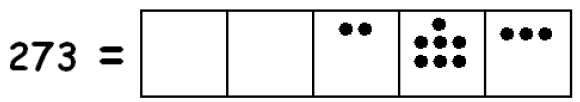
\includegraphics[height=2cm]{273base10}
\end{center}
And here is the number 512:
\begin{center}
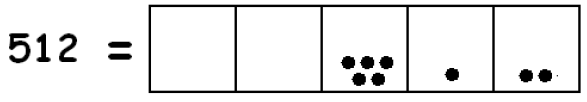
\includegraphics[height=2cm]{512base10}
\end{center}


\fellow{Most of these addition / subtraction examples might be nicer as animations, if we can do that!}

\begin{example}[$273+512$]
We can add these in the natural way: just combine the piles of dots.  Since they're already in place-value columns, we can combine dots from the two numbers that are in the same place-value box.
\begin{center}
\qquad\qquad\qquad\qquad
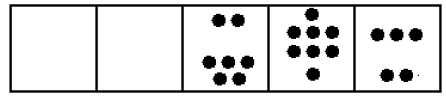
\includegraphics[height=2cm]{785base10}
\end{center}
We can count up the answer: there are 7 dots in the hundreds box, 8 dots in the tens box, and 5 dots in the ones box.

\begin{center}
\begin{tabular}{rl}
& 273\\
+ & 512\\ \hline
& 785
\end{tabular}
\end{center}

And saying out the long way we have:
\begin{itemize}
\item
Two hundreds plus five hundreds gives 7 hundreds.
\item
Seven tens plus one ten gives 8 tens.
\item
Three ones plus 2 ones gives 5 ones.
\end{itemize}
This is the answer 785.
\end{example}

\begin{example}[$163+489$]
Let's do another one.  Consider $163+489$.
\begin{center}
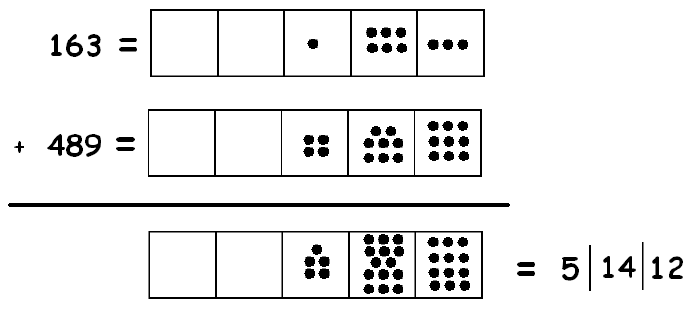
\includegraphics[height=5cm]{base10add1}

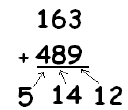
\includegraphics[height=2cm]{base10add2}
\end{center}

And this is absolutely mathematically correct:
\begin{itemize}
\item
One hundred plus four hundreds does give 5 hundreds.
\item
Six tens plus eight tens does give 14 tens.
\item
Three ones plus nine ones does give 12 ones.
\end{itemize}
The answer is $5 \mid 14 \mid 12$, which we might try to pronounce as``five hundred and
fourteeny-tenty twelvety!'' (Oh my!)

The trouble with this answer  is that most of the rest of the
world wouldn't understand what we are talking about! Since this is a base 10 system,
we can do some explosions.

\begin{center}
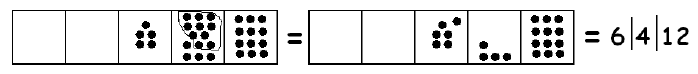
\includegraphics[height=1.4cm]{base10add3}
\end{center}
The answer now looks like ``six hundred forty twelvety''! Still not a familiar number, so let's do another
explosion:

\begin{center}
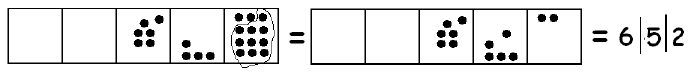
\includegraphics[height=1.5cm]{base10add4}
\end{center}
The answer is ``six hundred fifty two.'' Okay, the world can understand this one!
\begin{center}
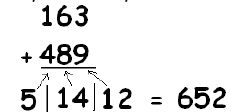
\includegraphics[height=2cm]{base10add5}
\end{center}
\end{example}


\begin{thinkpair*}
Solve the following exercises by thinking about the dots and boxes.
(You can draw the pictures, or just imagine them.) Then translate the answer into
something the rest of the world can understand.
\begin{center}
\begin{tabular}{rl}
& 148\\
+ & 323\\ \hline
\\
\end{tabular}
\qquad
\begin{tabular}{rl}
& 567\\
+ & 271\\ \hline
\\
\end{tabular}
\qquad
\begin{tabular}{rl}
& 377\\
+ & 188\\ \hline
\\
\end{tabular}
\qquad
\begin{tabular}{rl}
& 582\\
+ & 714\\ \hline
\\
\end{tabular}

\begin{tabular}{rl}
& 310462872\\
+ & 389107123\\ \hline
\\
\end{tabular}
\qquad
\begin{tabular}{cccccccccc}
& 872637163\\
+ & 187782748\\ \hline
\\
\end{tabular}

\end{center}
\end{thinkpair*}


\begin{problem}
Use the dots and boxes technique to solve these problems.  \emph{Do not convert to base 10!  Try to work directly in the base given.}  It might help to actually draw the pictures.

\begin{center}
\begin{tabular}{rl}
& $20413_\text{five}$ \\
+ & $13244_\text{five}$\\ \hline
\\
\end{tabular}
\qquad
\begin{tabular}{rl}
& $4052_\text{nine}$ \\
+ & $6288_\text{nine}$ \\ \hline
\\
\end{tabular}
\qquad
\begin{tabular}{rl}
& $3323_\text{seven}$ \\
+ & $3555_\text{seven}$ \\ \hline
\\
\end{tabular}
\end{center}

\end{problem}





\subsection{The Standard Algorithm for Addition}
Let's go back to the example $163 + 489$. Some teachers don't like writing:
\begin{center}
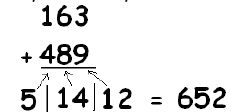
\includegraphics[height=2cm]{base10add5}
\end{center}

They prefer to teach their students to start with the 3 and 9 at the end and sum
those to get 12. This is of course correct --- we got 12 as well.
\begin{center}
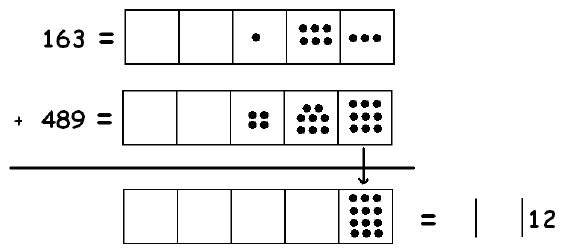
\includegraphics[height=5cm]{base10add6}
\end{center}
But they don't want students to write or think ``twelvety,''  so they have their students write something like this:
\begin{center}
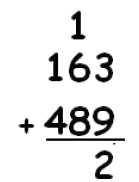
\includegraphics[height=2cm]{base10add8}
\end{center}
which can seem completely mysterious.
What's really going on?  They are exploding ten dots, of course!
\begin{center}
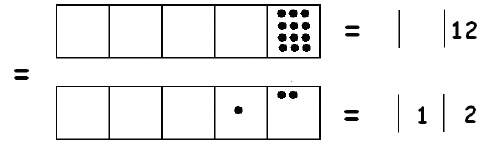
\includegraphics[height=3cm]{base10add7}
\end{center}

Now we carry on with the problem and add the tens.  Students are taught to write:
\begin{center}
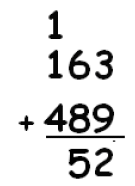
\includegraphics[height=2cm]{base10add10}
\end{center}
But what this means is better shown in this picture:
\begin{center}
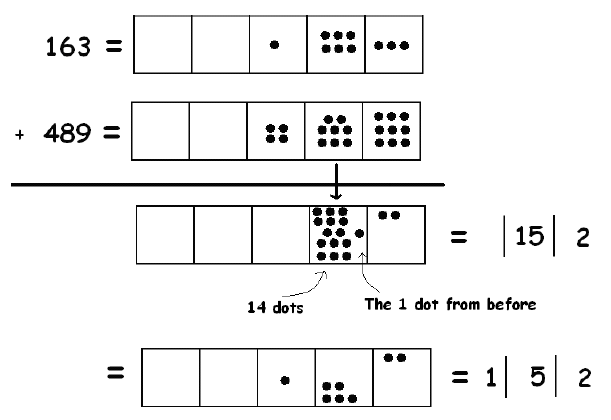
\includegraphics[height=7.5cm]{base10add9}
\end{center}

And now we finish the problem.
\begin{center}
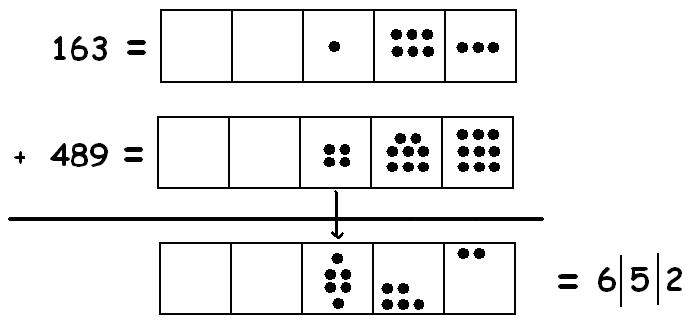
\includegraphics[height=5cm]{base10add11}

\bigskip
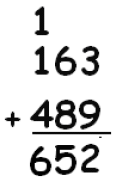
\includegraphics[height=2cm]{base10add12}

\end{center}


In the standard algorithm, we work from right to left, doing the ``explosions'' as we go along. This means
that we start adding at the ones place  and work towards the left-most place value,
``carrying'' digits that come from the explosions.  (This is really not carrying; a better for it is \emph{regrouping}.  Ten ones become one ten.  Ten tens become one hundred.  And so on.)

In the dots and boxes method, we add in any direction or order we like and then we do
the explosions at the end.
\begin{itemize}
\item
{\bf Why do we like the standard algorithm?}  Because it is efficient.
\item
{\bf Why do we like the dots and goes method?} Because it is easy to
understand.
\end{itemize}

\begin{thinkpair*}
Redo the problems below using the standard algorithm. You will see that
it is quicker.
\begin{center}
\begin{tabular}{rl}
& 148\\
+ & 323\\ \hline
\\
\end{tabular}
\qquad
\begin{tabular}{rl}
& 567\\
+ & 271\\ \hline
\\
\end{tabular}
\qquad
\begin{tabular}{rl}
& 377\\
+ & 188\\ \hline
\\
\end{tabular}
\qquad
\begin{tabular}{rl}
& 582\\
+ & 714\\ \hline
\\
\end{tabular}

\begin{tabular}{rl}
& 310462872\\
+ & 389107123\\ \hline
\\
\end{tabular}
\qquad
\begin{tabular}{cccccccccc}
& 872637163\\
+ & 187782748\\ \hline
\\
\end{tabular}
\end{center}

\end{thinkpair*}


\subsection{Subtraction as take-away}  In addition, we started with two collections of dots (two numbers), and we \emph{combined} them to form one bigger collection.  That's pretty much the definition of addition: combining two collections of objects.
  In subtraction, we start with one collection of dots (one number), and we take some dots away.


\begin{example}[$376-125$]
Suppose we want to find $376 - 125$ in the dots and boxes model.  We start with the representation of $376$:

\fellow{add picture of dots \& boxes for 376?}

Since we want to ``take away'' 125, that means we take away  one dot from the hundreds box, leaving two dots.  We take away two dots from the tens box, leaving five dots.  And we take away five dots from the ones box, leaving one dot.

\fellow{add picture of dots \& boxes for 251? Would be cool if we can see shadows or erasure of the 125.  If not, maybe an intermediate picture where the appropriate dots are circle with an arrow showing they're being removed?  (Sort of like pic at the bottom of p. 95 in the textbook, but using dots \& boxes) }

So the answer is:
\begin{center}
\begin{tabular}{rl}
&376 \\
$-$ & 125 \\ \hline
& 251
\end{tabular}
\end{center}


And saying out the long way we have:
\begin{itemize}
\item
Three hundreds take away one hundred leaves 2 hundreds.
\item
Seven tens take away two tens gives 5 tens.
\item
Six ones take away five  ones gives 1 one.
\end{itemize}

\end{example}


\begin{example}[$921 - 551$]
Let's try a somewhat harder example: $921-551$.  We start with the representation of $921$:

\fellow{add picture of dots \& boxes for 921?}

Since we want to ``take away'' 551, that means we take away  one dot from the hundreds box, leaving four dots.

\fellow{add picture of this?  }


  Now we want to take away five dots from the tens box, but we can't do it!  There are only two dots there.  What can we do?  Well, we still have some hundreds, so we can ``unexplode'' a hundreds dot, and put ten dots in the tens box instead.  Then we'll be able to take five of them away, leaving seven. 
    
  \fellow{add picture of this? show one of the hundreds dots being removed and becoming 10 tens dots, with arrows in the diagram somehow?}
  
   (Notice that we also have one less dot in the hundreds box; there's only three dots there now.)


    Now we want to take one dot from the ones box, and that leaves no dots there.
    
      \fellow{add picture of this?}

So the answer is:
\begin{center}
\begin{tabular}{rl}
&921 \\
$-$ & 551 \\ \hline
& 370
\end{tabular}
\end{center}

\end{example}


\begin{thinkpair*}
Solve the following exercises by thinking about the dots and boxes.
(You can draw the pictures, or just imagine them.) 

\begin{center}
\begin{tabular}{rl}
& 323\\
$-$ & 148\\ \hline
\\
\end{tabular}
\qquad
\begin{tabular}{rl}
& 567\\
$-$ & 271\\ \hline
\\
\end{tabular}
\qquad
\begin{tabular}{rl}
& 377\\
$-$ & 188\\ \hline
\\
\end{tabular}
\qquad
\begin{tabular}{rl}
& 714\\
$-$ & 582\\ \hline
\\
\end{tabular}

\begin{tabular}{rl}
& 389107123 \\
$-$ &310462872 \\ \hline
\\
\end{tabular}
\qquad
\begin{tabular}{cccccccccc}
& 872637163\\
$-$ & 187782748\\ \hline
\\
\end{tabular}

\end{center}
\end{thinkpair*}


\begin{problem}
Use the dots and boxes technique to solve these problems.  \emph{Do not convert to base 10!  Try to work directly in the base given.}  It will probably help to actually draw the pictures.

\begin{center}
\begin{tabular}{rl}
& $20413_\text{five}$ \\
$-$ & $13244_\text{five}$\\ \hline
\\
\end{tabular}
\qquad
\begin{tabular}{rl}
& $6288_\text{nine}$ \\
$-$ & $4052_\text{nine}$ \\ \hline
\\
\end{tabular}
\qquad
\begin{tabular}{rl}
& $3555_\text{seven}$ \\
$-$ & $3323_\text{seven}$ \\ \hline
\\
\end{tabular}
\end{center}

\end{problem}



\subsection{The Standard Algorithm for Subtraction}  Just like in addition, the standard algorithm for subtraction requires you to work from right to left, and ``borrow'' (this is really \emph{regrouping}!) whenever necessary.   Notice that in the dots and boxes approach, you don't need to go in any particular order when you do the subtraction.  You just ``unexplode'' the dots as necessary when computing.

Here's how the standard algorithm looks with the dots and boxes model for $921 - 551$:  Start with 921 dots.

\fellow{repeat the picture of 921 in dots \& boxes}

Then take away one dot from the ones box.


\fellow{show one dot going away}
\begin{center}
\begin{tabular}{rl}
&921 \\
$-$ & 551 \\ \hline
& \phantom{37}0
\end{tabular}
\end{center}


Now we want to take away five dots from the tens box.  But there aren't five dots there.  So we ``unexploded'' one of the hundreds dots to get more tens:

\fellow{picture of this?}

And here's how we're taught to write that regrouping:

\begin{center}
\begin{tabular}{rl}
&8 12\\
&\cancel{9}\ \cancel{2}\ 1 \\
$-$ & 5\ 5\ 1 \\ \hline
& \phantom{3\ 7\ }0
\end{tabular}
\end{center}
Now we have enough tens; we can take away five of them.
\begin{center}
\begin{tabular}{rl}
&8 12\\
&\cancel{9}\ \cancel{2}\ 1 \\
$-$ & 5\ 5\ 1 \\ \hline
& \phantom{3\ }7\ 0
\end{tabular}
\end{center}

Finally, we want to take away five hundreds.

\fellow{picture of this?}

\begin{center}
\begin{tabular}{rl}
&8 12\\
&\cancel{9}\ \cancel{2}\ 1 \\
$-$ & 5\ 5\ 1 \\ \hline
& 3\ 7\ 0
\end{tabular}
\end{center}



\subsection{Multiplication as Repeated Addition}

\begin{problem}\label{prob:dotsmultiply}
Jenny was asked to compute $243192\times 4$. She wrote:

\begin{center}
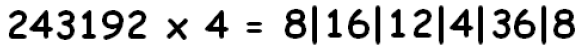
\includegraphics[height=1cm]{mult1}
\end{center}

\begin{enumerate}[(a)]
\item
What was Jenny thinking about? Is her answer correct?

\item
Translate Jenny's answer into a number that the rest of the world can
understand.

\item
Use Jenny's method to find the answers to these multiplication exercises.  Be sure to translate your answers into familiar base 10 numbers.

\[
156 \times 3 = 
\qquad\qquad
2873 \times 2 = 
\qquad\qquad
71181\times 5 = 
\qquad\qquad
3726510392 \times 2 = 
\quad
\]
\end{enumerate}

\begin{problem}\label{prob:dotsmultiplybase8}
Can you adapt Jenny's method to solve these problems?  Write your answers in base eight.  Try to work directly in base eight rather than converting to base 10 and back again!

\[
156_\text{eight} \times 3_\text{eight} = 
\qquad\qquad
2673_\text{eight} \times 4_\text{eight} = 
\qquad\qquad
36255772 \times 2_\text{eight} = 
\quad
\]

\end{problem}

\begin{thinkpair*}
After you have worked on  problems \ref{prob:dotsmultiply} and \ref{prob:dotsmultiplybase8}, share your ideas with a partner.   Can you relate Jenny's method to the standard algorithm for multiplication?
\end{thinkpair*}


Jenny  might have been thinking about multiplication as repeated addition.  If we have some number $N$ and we multiply that number by 4, what we mean is:
\[
4 \cdot N = N + N + N + N.
\]

If we take the number  $243192$ and add it to itself four times using the ``combining method,'' we get $2+2+2+2 = 8$ ones, $9+9+9+9 = 36$ tens, $1+1+1+1 = 4$ hundreds, and so on.


{\bf Notation:}
Notice that we have used both $\times$ and $\cdot$ to represent multiplication.  It's a bit awkward to use $\times$ when you're also using variables.  Is it the letter $x$?  Or the multiplication symbol $\times$?  It can be hard to tell!  In this case, the symbol $\cdot$ is  more clear.  We can even simplify the notation further, writing $4N$ instead of $4 \cdot N$.  But of course we \emph{only} do that when we are multiplying variables by some quantity.  (We wouldn't want $34$ to mean $3 \cdot 4$, would we?)


\begin{problem}
Here is a strange addition table.  Use it to solve the following problems.    \emph{Important: Don't try to assign numbers to $A$, $B$, and $C$.  Solve the problems just using what you know about the operations!}

\begin{center}
\begin{tabular}{c | c c c}
\quad $+$ \quad  & \quad $A$ \quad &\quad $B$ \quad&\quad $C$\quad \\ \hline
& \\
$A$ & $C$ &$A$ & $B$ \\
& \\
$B$ & $A$ &$B$ & $C$ \\
& \\
$C$ & $B$ &$C$ & $A$ \\
\end{tabular}
\end{center}

\[
A + B
\qquad\qquad
B+ C
\qquad\qquad
2 A
\qquad\qquad
5 C
\qquad\qquad
3 A + 4 B
\]

\end{problem}

\end{problem}


\begin{thinkpair*}
Discuss your answers with a partner.  How does an addition table help you solve multiplication problems like $5  C$?
\end{thinkpair*}




\subsection{Quotative Model of Division}
Suppose you are asked to compute $3906 \div 3$.  One way to interpret this question (there are others) is:
\begin{quote}
``How many groups of 3 fit into 3906?''
\end{quote}

\begin{define}
In the \emph{quotative} model of division, you are given a \emph{dividend} (here it is 3906), and you are asked to split it into equal-sized groups, where the size of the group is given by the \emph{divisor} (here it is 3).
\end{define}

In our dots and boxes model, the dividend 3906 looks like this:
\begin{center}
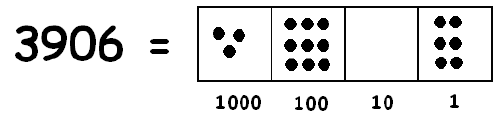
\includegraphics[height=2cm]{divide1}
\end{center}
and three dots looks like this:

\includegraphics[height=.4cm]{divide2}.
So we are really asking:

\begin{quote}
``How many groups of 
\includegraphics[height=.4cm]{divide2} fit into the picture of 3906?''
\end{quote}

There is  one group of 3 at the thousands level, and three at the hundreds level,
none at the tens level, and two at the ones level.
\begin{center}
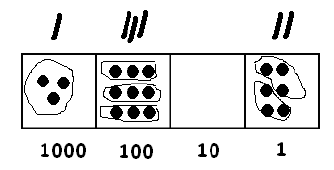
\includegraphics[height=3cm]{divide3}
\end{center}

Notice what we have in the picture:
\begin{itemize}
\item
One group of 3 in the thousands box.
\item
Three groups of 3 in the hundreds box.
\item
Zero groups of 3 in the tens box.
\item
Two groups of 3 in the ones box.
\end{itemize}
This shows that 3 goes into 3906 one thousand, three hundreds and two ones times. 
That is,
\[
3906 \div 3 = 1302.
\]

{\bf Fun fact:} The division sign $\div$ has an unusual name. It is called an
\emph{obelus}. Not many people know this.

Let's try a harder one! Consider $402 \div 3$.
  Here's the picture:
  \begin{center}
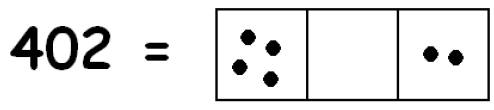
\includegraphics[height=1.5cm]{divide4}
\end{center}

  
  We are still looking for groups of three dots: 
\includegraphics[height=.4cm]{divide2}.


There is certainly one group at the 100s level.
  \begin{center}
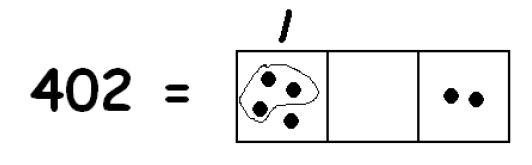
\includegraphics[height=2cm]{divide5}
\end{center}
and now it seems we are stuck � there are no more groups of three!


\begin{thinkpair*}
What can we do now? Are we really stuck?  Can you finish the division problem?  
\end{thinkpair*}


\begin{example}[$402\div 3$]
Here are the details worked out for $402 \div 3$.  But don't read this until you've thought about it yourself!

Since each dot is worth ten dots in the box to the right we can write:
  \begin{center}
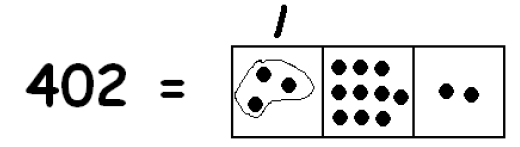
\includegraphics[height=2cm]{divide6}
\end{center}
Now we can find more groups of three:
  \begin{center}
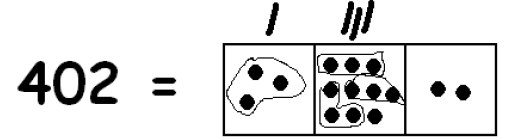
\includegraphics[height=1.9cm]{divide7}
\end{center}
There is still a troublesome extra dot. Let's unexploded it too
  \begin{center}
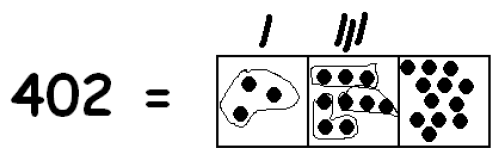
\includegraphics[height=2.2cm]{divide8}
\end{center}
This gives us more groups of three:
  \begin{center}
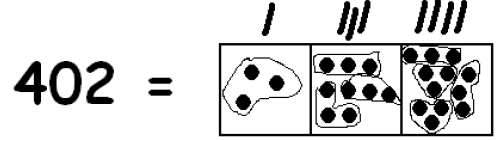
\includegraphics[height=2cm]{divide9}
\end{center}

In the picture we have:
\begin{itemize}
\item
One group of 3 in the hundreds box.
\item
Three groups of 3 in the tens box.
\item
Four groups of 3 in the ones box.
\end{itemize}
Finally we have the answer!  
\[
402 \div 3 = 134.
\]

\end{example}

\begin{thinkpair*}
Solve each of these exercises using the dots and boxes method:
\[
62124 \div 3 
\qquad
\qquad
\qquad
61230 \div 5
\]

\end{thinkpair*}


Let's turn up the difficulty a notch.   Consider $156 \div 12$.
Here we are looking for groups of 12 in this picture:
  \begin{center}
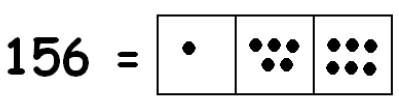
\includegraphics[height=1.5cm]{divide10}
\end{center}

What does 12 look like?  It can be twelve dots in a single box:
  \begin{center}
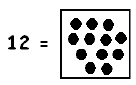
\includegraphics[height=1.7cm]{divide11}
\end{center}
But most often we would write 12 this way:
  \begin{center}
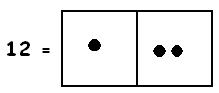
\includegraphics[height=1.7cm]{divide12}
\end{center}
We certainly see some of these in the picture. There is certainly one at the tens
level:
  \begin{center}
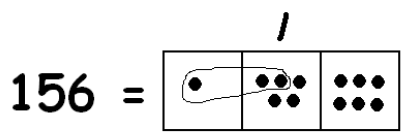
\includegraphics[height=2.2cm]{divide13}
\end{center}

(REMEMBER: With an unexplosion this would be twelve dots in the tens box.)


And three at the ones level:
  \begin{center}
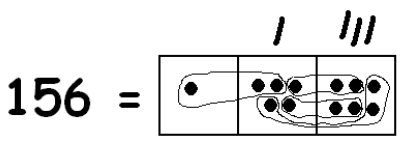
\includegraphics[height=2.2cm]{divide14}
\end{center}

So in the picture we have:
\begin{itemize}
\item
One group of 12 dots in the tens box.
\item
Three groups of 12 dots in the ones box.
\end{itemize}
That means
\[
156 \div 12 = 13.
\]

\begin{problem}\label{prob:practicediv}
Use the dots and boxes model to compute each of the following:
\[
13453 \div 11
\qquad\qquad
4853 \div 23
\qquad\qquad
214506 \div 102
\]


\end{problem}


\begin{thinkpair*}\ 
\begin{itemize}
\item
Compare your solutions to problem \ref{prob:practicediv} with a partner.  

\item
When you agree that you are doing the process correctly, use dots and boxes to compute these:

\[
2130 \div 10
\qquad\qquad
41300 \div 100
\]

\item
Discuss: What pictures did you use for 10 and for 100? Can you describe in words what happens
when dividing by 10 and by 100 and \emph{why}?
\end{itemize}
\end{thinkpair*}



\subsection{The Standard Algorithm for Division}
We used dots and boxes to show that $402 \div 3 = 134$.
  \begin{center}
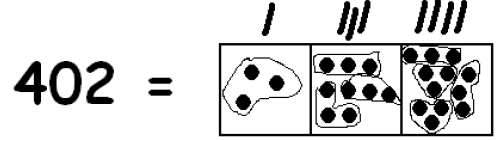
\includegraphics[height=2cm]{divide9}
\end{center}


In elementary school, you might have learned to solve this division problem by using a diagram
like the following:
  \begin{center}
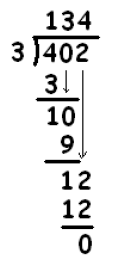
\includegraphics[height=4cm]{divide15}
\end{center}
At first glance this seems very mysterious, but it is really no different from the
dots and boxes method. Here is what the table means.

To compute $402 \div 3$, we first make a big estimation as to how many groups of
3 there are in 402. Let's guess that there are 100 groups of three.
  \begin{center}
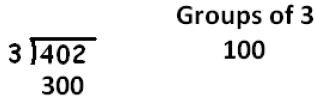
\includegraphics[height=2cm]{divide16}
\end{center}
How much is left over after taking away 100 groups of 3?
  \begin{center}
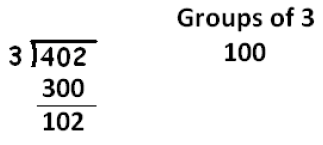
\includegraphics[height=2.4cm]{divide17}
\end{center}
How many groups of 3 are in 102? Let's try 30:
  \begin{center}
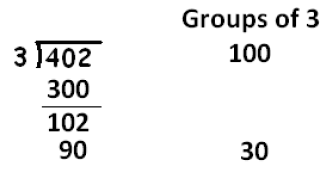
\includegraphics[height=2.8cm]{divide18}
\end{center}
How many are left? There are 12 left and there are four groups of 3 in 12.
  \begin{center}
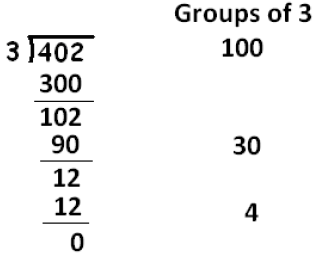
\includegraphics[height=4cm]{divide19}
\end{center}
The accounts for entire number 402. And where doe we find the final answer? Just
add the total count of groups of three that we tallied:
\[
402 \div 3 = 100 + 30 + 4 = 134.
\]


\begin{thinkpair*}
Compare these two diagrams.  In what way are they the same? In what way are they different?
  \begin{center}
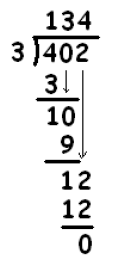
\includegraphics[height=4cm]{divide15}
\qquad\qquad\qquad\qquad\qquad\qquad
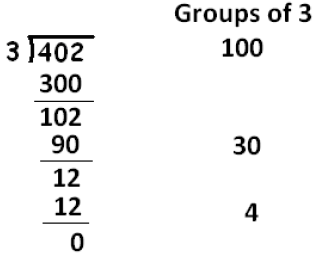
\includegraphics[height=4cm]{divide19}
\end{center}


Look at the dots and boxes method.  In what way is the same or different from the two tables?
  \begin{center}
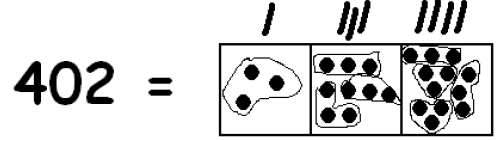
\includegraphics[height=2cm]{divide9}
\end{center}

\end{thinkpair*}


\begin{itemize}
\item
{\bf Why do we like the standard algorithm?}   Because it is quick, not too much to
write down, and it works.
\item
{\bf Why do we like the dots and boxes method?}   Because it easy to
understand. (And drawing dots and boxes is kind of fun!)
\end{itemize}


We saw that 402 is evenly divisible by 3: $ 402 \div 3 = 134$.  This means that 403, one more, shouldn't be divisible by three. It should be one dot
too big. Do we see the extra dot if we try the dots and boxes method?
  \begin{center}
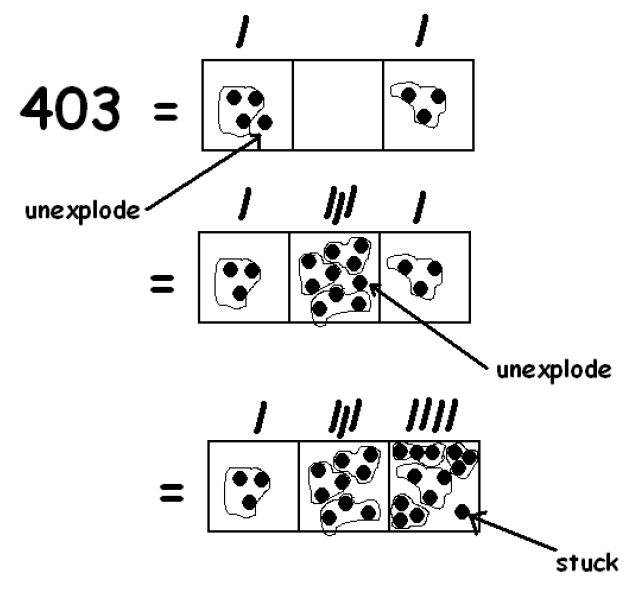
\includegraphics[height=9cm]{divide20}
\end{center}
Yes we do! We have  one dot left at the end that can't be divided. We say that we
have a \emph{remainder} of one and some people like to write:
\[
403 \div 3 = 134\  R1.
\]


Let's try another one: $263 \div 12$.  Here's what we have:
  \begin{center}
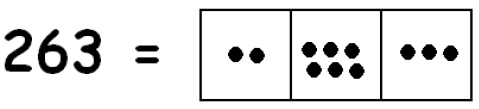
\includegraphics[height=2cm]{divide21}
\end{center}
And we are looking for groups like this:
  \begin{center}
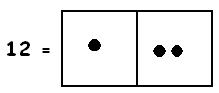
\includegraphics[height=2cm]{divide12}
\end{center}
Here goes!
  \begin{center}
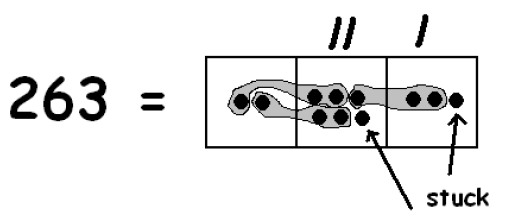
\includegraphics[height=4cm]{divide22}
\end{center}
Unexploding won't help any further and we are indeed left with one remaining dot in
the tens position and a dot in the ones position. This means we
have a remainder of eleven.
\[
263 \div 12 = 21\ R 11.
\]

\begin{thinkpair*}\ 
\begin{itemize}
\item
Use the dots and boxes method to compute each quotient:
\[
5210 \div 4
\qquad\qquad
4857 \div 23
\qquad\qquad
31533 \div101
\]

\item
Now use the standard algorithm (an example is  shown below) to compute each of the quotients above.
  \begin{center}
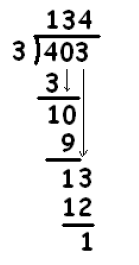
\includegraphics[height=5cm]{divide23}\\
$403 \div 3 = 134\ R1$.
\end{center}

\item
Which method do you like better: dots and boxes or the standard algorithm method? Or does
it depend on the problem you are doing?  
\end{itemize}
\end{thinkpair*}


\begin{thinkpair*}
Which is the \emph{best} explanation for why this long division algorithm works? Think about your choice on your own.  Then share your choice with a partner and see if you can agree on the best answer.  


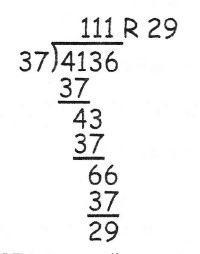
\includegraphics[height=5 cm]{LongDiv}
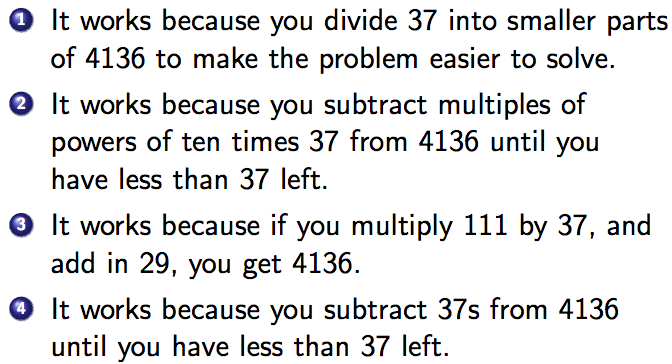
\includegraphics[height=5 cm]{DivExplain}
\end{thinkpair*}







\section{Model 2: Measurement}
Another way we often think about numbers is as abstract quantities that can be measured: length, area, and volume are all examples.

\begin{thinkpair*}
Answer the following questions about each picture:
\begin{itemize}
\item
If $A = 1$ unit, then what numbers would you assign to $B$ and $C$?  Why?
\item
If $B = 1$ unit, then what numbers would you assign to $A$ and $C$?  Why?
\end{itemize}

\begin{center}
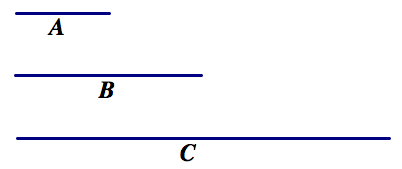
\includegraphics[height = 2.75cm]{length}
\qquad\qquad
\includegraphics[height = 3.25cm]{area}

\fellow{can you make up a similar picture for volume?  maybe that one is too hard?  If it doesn't work, don't worry about it.}
\end{center}

\end{thinkpair*}

In a measurement model, you have to pick a \emph{basic unit}.  The basic unit is a quantity --- length, area, or volume --- that you assign to the number one.  You can then assign numbers to other quantities based on how many of your basic unit fit inside. 

For now, we'll focus on the quantity \emph{length}, and we'll work with a number line where the basic unit is already marked off.
\begin{center}
\includegraphics[height = 2.5cm]{numberline1}
\end{center}



\subsection{Addition and Subtraction on the Number Line}
Imagine a person --- we'll call him Zed --- who can stand on the number line.  We'll say that the distance Zed walks when he takes a step is exactly one unit.

\fellow{any chance of a picture of a person on the number line?  I can do a terrible stick figure, but maybe you can do something better?}

When Zed wants to add or subtract with whole numbers on the number line, he always starts at 0 and faces the positive direction (towards 1).  Then what he does depends on the calculation.

If Zed wants to \emph{add} two numbers, he walks forward (to the right of the number line)  however many steps are indicated by the first number (the first \emph{addend}).  Then he walks forward (to your right on the number line) the number of steps indicated by the second number (the second \emph{addend}).  Where he lands is the \emph{sum} of the two numbers.

\begin{example}[$3+4$]
If Zed wants to add $3+4$, he starts at 0 and faces towards the positive numbers.  He walks forward  3 steps, then he walks forward  4 more steps.  

\fellow{picture?  or even better an animation?}

Zed ends at the number 7, so the sum of 3 and 4 is 7.  $3+4 = 7$.  (But you knew that of course!  The point right now is to make sense of the \emph{number line model}.)
\end{example}


When Zed wants to \emph{subtract} two numbers, he he walks forward (to the right on the number line)  however many steps are indicated by the first number  (the  \emph{minuend}).  Then  he walks \emph{backwards} (to the left on the number line) the number of steps indicated by the second number (the  \emph{subtrahend}).  Where he lands is the \emph{difference} of the two numbers.


\begin{example}[$11 - 3$]
If Zed wants to subtract $11-3$, he starts at 0 and faces the positive numbers (the right side of the number line).
He walks forward 11 steps on the number line, then he walks backwards 3 steps.  

\fellow{picture?  or even better an animation?}

Zed ends at the number 8, so the difference of 11 and 3 is 8.  $11-3 = 8$.  (But you knew that!)
\end{example}




\begin{thinkpair*}\ 
\begin{itemize}
\item
Work out each of these exercises on a number line.  You can actually pace it out on a life-sized number line or draw a picture:
\[
4 + 5 
\qquad\qquad
6 + 9
\qquad\qquad
10-7
\qquad\qquad
8-1
\]

\item
Why does it make sense to walk forward for addition and walk backwards for subtraction?  In what way is this the same as ``combining'' for addition and ``take away'' for subtraction''?

\item
What happens if you do these subtraction problems on a number line?    Explain your answers.
\[
6 - 9
\qquad\qquad
1-7
\qquad\qquad
4 - 11 
\qquad\qquad
0-1
\]

\item
Could you do the subtraction problems above with the dots and boxes model?  


\end{itemize}

\end{thinkpair*}






\subsection{Multiplication and Division on the Number Line}
Since  multiplication is really repeated addition, we can adapt our addition model to become a multiplication model as well.  Let's think about $3 \times 4$.  This means to add four to itself three times (that's simply the definition of multiplication!):
\[
3 \times 4 = 4 + 4 + 4.
\]
So to multiply  on the number line, we do the process for addition several times.

To multiply two numbers, Zed starts at 0 as always, and he faces the positive direction.  He walks forward the number of steps given by the second number (the second \emph{factor}).  He repeats that process the number of times given by the first number (the first \emph{factor}).  Where he lands is the \emph{product} of the two numbers.


\begin{example}[$3\times 4$]
If Zed wants to multiply $3\times 4$, he can think of it this way:
\[
\underbrace{3}_\text{how many times to repeat it} \times \underbrace{4}_\text{how many steps to take forward}
\]
Zed starts at 0, facing the positive direction.  The he repeats this three times: take four steps forward.

\fellow{picture? or animation?}

He ends at the number 12, so the product of 3 and 4 is 12.  That is, $3 \times 4 = 12$.
\end{example}



Remember our quotative model of division:  One way to interpret  $15 \div 5$ (there are others) is:
\begin{quote}
``How many groups of 5 fit into 15?''
\end{quote}
Thinking on the number line, we can ask it this way:
\begin{quote}
``Zed takes 5 steps at a time.  If Zed lands at the number 15, how many times did he take 5 steps?''
\end{quote}

To calculate a division problem on the number line, Zed starts at 0, facing the positive direction.  He walks forward the number of steps given by the second number (the \emph{divisor}).  He repeats that process until he lands at the first number (the \emph{dividend}).  The number of times he repeated the process gives the \emph{quotient} of the two numbers.



\begin{example}[$15\div 5$]
If Zed wants to divide $15 \div 5$, he can think of it this way:
\[
\underbrace{15}_\text{where he wants to land} \div \underbrace{5}_\text{how many steps he takes at a time}
\]
He starts at 0, facing the positive direction.
\begin{itemize}
\item
Zed takes 5 steps forward.  He is now at 5, not 15.  So he needs to repeat the process.
\item
Zed takes 5 steps forward again.  He is now at 10, not 15.  So he needs to repeat the process.
\item
Zed takes 5 more steps forward.  He is at 15, so he stops.
\end{itemize}

\fellow{animation?  or picture for each bullet point? or at least one picture showing the whole process?}

Since he repeated the process three times, we see there are 3 groups of 5  in 15.
So the quotient of 15 and 5 is 3.  That is, $15 \div 5 = 3$.
\end{example}




\begin{thinkpair*}\ 
\begin{itemize}
\item
Work out each of these exercises on a number line.  You can actually pace it out on a life-sized number line or draw a picture:
\[
2 \times 5
\qquad\quad
7 \times 1
\qquad\quad
10 \div 2
\qquad\quad
6 \div 1
\]


\item
Can you think of a way to interpret these multiplication problems on a number line?    Explain your ideas.
\[
4 \times 0
\qquad\qquad
0 \times 5
\qquad\qquad
3 \times (-2)
\qquad\qquad
2 \times (-1)
\]

\item
What happens if you try to solve these division problems on a number line?  Can you do it?    Explain your ideas.
\[
0 \div 2
\qquad\qquad
0 \div 10
\qquad\qquad
3 \div 0
\qquad\qquad
5 \div 0
\]

\end{itemize}

\end{thinkpair*}

 




\subsection{Area Model for Multiplication}
So far we have focused on a \emph{linear} measurement model, using the number line.  But there's another common way to think about multiplication: using \emph{area}.

For example, suppose our basic unit is one square:

\begin{center}
\includegraphics[height=1cm]{basicsquare}
\end{center}

We can picture $4 \times 3$ as 4 groups, with 3 squares in each group, all lined up:

\begin{center}
\includegraphics[height=1cm]{3squares}
\includegraphics[height=1cm]{3squares}
\includegraphics[height=1cm]{3squares}
\includegraphics[height=1cm]{3squares}
\end{center}


But we can also picture  them stacked up instead of lined up.  We would have 4 \emph{rows}, with 3 squares in each \emph{row}, like this:
\begin{center}
\includegraphics[height=4cm]{4x3squares}
\end{center}


So we can think about $4 \times 3$ as a rectangle that has length 3 and width 4.  The product, 12, is the total number of squares in that rectangle.  (That is also the \emph{area} of the rectangle, since each square was one unit!)

\begin{thinkpair*}
Vera drew this picture as a model for $15\times 17$.  Use her picture to help you compute $15\times 17$.  Explain your work.
\begin{center}
\includegraphics[height=3.5cm]{15x17}
\end{center}
\end{thinkpair*}
 
 
 \begin{problem}
 Draw pictures like Vera's for each of these multiplication exercises.  Use your pictures to find the products without using a calculator or the standard algorithm.
 
 \[
 23 \times 37 
 \qquad\qquad
 8 \times 43
 \qquad\qquad
 371\times 42
 \]
 \end{problem}


\subsection{The Standard Algorithm for Multiplication}
How were you taught to compute $83\times 27$ in school? Were you taught
to write something like the following?

\begin{center}
\begin{tabular}{rl}
&$\phantom{22}83$\\
$\times$&$\phantom{22}27$\\\hline
&$\phantom{22}21$\\
&$\phantom{2}56$\\
&$\phantom{22}6$\\
&$16$\\\hline
&$2241$
\end{tabular}
\end{center}
Or maybe you were taught to put in the extra zeros rather than leaving them out?
\begin{center}
\begin{tabular}{rl}
&$\phantom{22}83$\\
$\times$&$\phantom{22}27$\\\hline
&$\phantom{22}21$\\
&$\phantom{2}560$\\
&$\phantom{22}60$\\
&$1600$\\\hline
&$2241$
\end{tabular}
\end{center}

This is really no different than drawing the rectangle and using Vera's shortcut for calculating!
\begin{center}
\includegraphics[height=5cm]{83x27}
\end{center}

\begin{thinkpair*}\ 
\begin{itemize}
\item
Use the example above to explain why Vera's rectangle method and the standard algorithm are really the same.

\item
Calculate the products below using both methods.  Explain where you're computing the same pieces in each algorithm.
\[
23 \times 14
\qquad\qquad
106 \times 21
\qquad\qquad
213\times 31
\]

\end{itemize}
\end{thinkpair*}


\begin{problem}[Lines and Intersections]
Here's an unusual way to perform long multiplication. To compute $22\times13$, for
example, draw two sets of vertical lines, the left set containing two lines and the
right set two lines (for the digits in 22) and two sets of horizontal lines, the upper
set containing one line and the lower set three (for the digits in 13).

\begin{center}
\includegraphics[height=5cm]{lines1}
\end{center}

There are four sets of intersection points. Count the number of intersections in
each and add the results diagonally as shown:

\begin{center}
\includegraphics[height=5cm]{lines2}
\end{center}
The answer 286 appears!

There is one possible glitch as illustrated by the computation $246\times  32$:
\begin{center}
\includegraphics[height=5cm]{lines3}
\end{center}

Although the answer 6 thousands, 16 hundreds, 26 tens, and 12 ones is absolutely
correct, one needs to carry digits and translate this as $7,872$.

\begin{enumerate}[(a)]
\item
Compute $131\times 122$ via this method.  Check your answer using another method.

\item
Compute $15\times 1332$ via this method.  Check your answer using another method.


\item
Can you adapt the method to compute $102\times 3054$?  (Why is some adaptation necessary?)

\item
Why does the method work in general?
\end{enumerate}

\end{problem}






\begin{problem}[Lattice Multiplication]
In the 1500s in England, students were taught to compute long multiplication using
following galley method, now more commonly  known as the \emph{lattice method}:

To multiply 43 and 218, for example, draw a $2\times 3$ grid of squares. Write the digits
of the first number along the right side of the grid and the digits of the second number
along the top. 

Divide each cell of the grid diagonally and write in the product
of the column digit and row digit of that cell, separating the tens from the units
across the diagonal of that cell. (If the product is a one digit answer, place a 0 in
the tens place.)

\begin{center}
\includegraphics[height=5cm]{latticemult}
\end{center}


Add the entries in each diagonal, carrying tens digits over to the next diagonal if
necessary, to see the final answer. In our example, we have $218\times 43 = 9374$.


\begin{enumerate}[(a)]
\item
Compute $5763\times 345$ via the lattice method.
\item Explain why the lattice method is really the standard algorithm  in disguise. 
\item
What is the
specific function of the diagonal lines in the grid?


\end{enumerate}

\end{problem}









\section{Operations}
So far, you have seen a couple of different \emph{models} for the operations: addition, subtraction, multiplication, and division.  But we haven't talked much about the operations themselves --- how they relate to each other, what properties they have that make computing easier, and how some special numbers behave.  There's lots to think about!

The goal in this section is to use the models to understand why the operations behave according to the rules you learned back in elementary school.  We're going to keep asking ourselves ``Why does it work this way?''



\begin{thinkpair*}
Each of these models lends itself to thinking about the operation in a slightly different way.  Before we really dig in to thinking about the operations, discuss with a partner:
\begin{itemize}
\item
Of the models we discussed so far, do you prefer one of them?
\item
How well do the models we discussed match up with how you usually think about whole numbers and their operations?
\item
Which models are useful for computing?  Why?
\item
Which models do you think will be useful for \emph{explaining} how the operations work?  Why?
\end{itemize}
\end{thinkpair*}


\subsection{Relationships Between the Operations}
We defined addition as combining two quantities and subtraction as ``taking away.'' But in fact, these two operations are intimately tied together.  These two questions are exactly the same:
\[
27 - 13 = \underline{\qquad}
\qquad\qquad
27 = 13 + \underline{\qquad}.
\]
More generally, for any three whole numbers $a$, $b$, and $c$, these two equations express the  same fact.  (So either both equations are true or both are false.  Which is the case depends on the values you choose for $a$, $b$, and $c$!)
\[
c - b = a
\qquad\qquad
c = a+ b.
\]
In other words, we can think of every subtraction problem as a ``missing addend'' addition problem.  Try it out!

\begin{problem}
Here is a strange addition table.  Use it to solve the following problems.  Justify your answers.  \emph{Important: Don't try to assign numbers to $A$, $B$, and $C$.  Solve the problems just using what you know about the operations!}

\begin{center}
\begin{tabular}{c | c c c}
\quad $+$ \quad  & \quad $A$ \quad &\quad $B$ \quad&\quad $C$\quad \\ \hline
& \\
$A$ & $C$ &$A$ & $B$ \\
& \\
$B$ & $A$ &$B$ & $C$ \\
& \\
$C$ & $B$ &$C$ & $A$ \\
\end{tabular}
\end{center}

\[
A+ C 
\qquad\qquad
B + C
\qquad\qquad
A - C
\qquad\qquad
C - A
\qquad\qquad
A - A
\qquad\qquad
B - C
\]


\end{problem}


\begin{thinkpair*}
Discuss your answers with a partner.  How does an addition table help you solve subtraction problems?
\end{thinkpair*}


We defined multiplication as repeated addition and division as forming groups of equal size. But in fact, these two operations are also tied together.  These two questions are exactly the same:
\[
27 \div 3 = \underline{\qquad}
\qquad\qquad
27 =  \underline{\qquad} \times 3.
\]
More generally, for any three whole numbers $a$, $b$, and $c$, these two equations express the  same fact.  (So either both equations are true or both are false.  Which is the case depends on the values you choose for $a$, $b$, and $c$!)
\[
c \div b = a 
\qquad\qquad
c = a \cdot b.
\]
In other words, we can think of every division problem as a ``missing factor'' multiplication problem.  Try it out!


\begin{problem}\label{prob:divby0}
Rewrite each of these division problems as a ``missing factor'' multiplication problem.  Which ones can you solve and which can you not solve?  Explain your answers.
\[
9 \div 3 
\qquad\qquad
100 \div 25
\qquad\qquad
0 \div 3
\qquad\qquad
9 \div 0
\qquad\qquad
0 \div 0
\]
\end{problem}



\begin{problem}\label{prob:divmulttable}
Here's a multiplication table.  

\begin{center}
{\large
\begin{tabular}{c|| c |c|c|c|c}
 \quad $\times$ \quad & \quad $a$ \quad &  \quad $b$ \quad  &  \quad $c$ \quad  
 & \quad $d$ \quad  &  \quad $e$ \quad   \\ \hline\hline
 & & & & &  \\
$a$ & $a$ & $a$ & $a$ & $a$& $a$ \\ \hline
 & & & & &  \\
$b$ & $a$ & $b$ & $c$ & $d$ & $e$\\ \hline
 & & & & &  \\
$c$ & $a$ & $c$ & $e$ & $b$ & $d$\\ \hline
 & & & & &  \\
$d$ & $a$ & $d$ & $b$ & $e$ & $c$\\ \hline
 & & & & & \\
$e$& $a$ & $e$ & $d$ & $c$ & $b$\\ 
\end{tabular}}
\end{center}

\begin{itemize}
\item
Use the table to solve the problems below.  Justify your answers.    \emph{Important: Don't try to assign numbers to the letters.  Solve the problems just using what you know about the operations!}
\[
c\times d 
\qquad\qquad
c\times a 
\qquad\qquad
a\times a 
 \qquad\qquad
c \div d
\qquad\qquad
d \div c
\qquad\qquad
d \div e
\]

\item
Can you use the table to solve these problems?  Explain your answers.
\[
d^2
\qquad\qquad
c^3
\qquad\qquad
a \div c
\qquad\qquad
a \div d
 \qquad\qquad
c \div a
\qquad\qquad
d \div a
\qquad\qquad
a \div a
\]
\end{itemize}

\end{problem}


\begin{thinkpair*}
Discuss your answers to problems \ref{prob:divby0} and \ref{prob:divmulttable} with a partner.  How does a multiplication table help you solve division (and exponentiation) problems?
\end{thinkpair*}




Throughout this course, our focus is on explanation and justification.  As teachers, you need to know what is true in mathematics, but you also need to know \emph{why} it is true.  And you will need lots of ways to explain \emph{why}, since different explanations will make sense to different students.

It's very important not to confuse the fact (or rule) with the reason it is true!  Here are some examples:

\begin{example}[Explaining the Connection Between Addition and Subtraction]\ 

{\bf Arithmetic Fact:} $a + b = c$ and $c - b = a$ are the same mathematical fact.

{\bf Why It's True, Explanation 1:} First we'll use the definition of the operations.  

 Suppose we know $c-b = a$ is true.   Subtraction means ``take away.''  So 
 \[
 c - b = a
 \]
  means we start with quantity $c$ and take away quantity $b$, and we end up with quantity $a$.  Start with this equation, and imagine adding quantity $b$ to both sides. 
  
  On the left, that mans we started  with quantity $c$, took away $b$ things, and then put those $b$ things right back! Since we took away some quantity and then added back the exact same quantity, there's no overall change.  We're left with quantity $c$.
  
    
  On the right, we would be \emph{combining} (adding) quantity $a$ with quantity $b$.   So we end up with
  \[
  c = a+b.
  \]
  
  On the other hand, suppose we know the equation $a + b = c$ is true.  Imagine \emph{taking away} (subtracting) quantity $b$ from both sides of the equation
  \[
  a+b = c.
  \]
 On the left, we started with $a$ things and \emph{combined} that with  $b$ things, but then we immediately take away those $b$ things.  So we're left with just our original quantity of $a$.    
 
 On the right, we start with quantity $c$ and \emph{take away} $b$ things.  That's the very definition of $c-b$.  So we have the equation
 \[
a = c- b.
 \]
 
 \fellow{Maybe this would be  more clear as an animation!}



{\bf Why It's True, Explanation 2:} Let's use the measurement model to come up with another explanation.  

The equation $a + b = c$  means Zed starts at 0, walks forward $a$ steps, and then walks forward $b$ steps, and he ends at $c$.

If Zed wants to compute $c - b $, he starts at 0, walks forward $c$ steps, and then walks backwards $b$ steps.
But we know that to walk forward  $c$ steps, he can first walk forward $a$ steps and then walk forward $b$ steps.  So Zed can compute $c - b$ this way: 
\begin{itemize}
\item
Start at 0.
\item
Walk forward $a$ steps.
\item
Walk forward $b$ steps.  (Now at $c$, since $a + b = c$.)
\item
Walk backwards $b$ steps.
\end{itemize}

\fellow{picture?}

The last two steps cancel each other out, so Zed lands back at $a$.  That means $c-b = a$.

On the other hand, the equation $c - b = a$ means that Zed starts at 0, walks forward $c$ steps, then walks backwards $b$ steps, and he ends up at $a$.

If Zed wants to compute $a+ b $, he starts at 0, walks forward $a$ steps, and then walks forwards $b$ additional steps.
But we know that to walk forward  $a$ steps, he can first walk forward $c$ steps and then walk backwards $b$ steps.  So Zed can compute $a + b$ this way: 
\begin{itemize}
\item
Start at 0.
\item
Walk forward $c$ steps.
\item
Walk backwards $b$ steps.  (Now at $a$, since $c-b = a$.)
\item
Walk forward $b$ steps.
\end{itemize}
\fellow{picture?}


The last two steps cancel each other out, so Zed lands back at $c$.  That means $a+b = c$.

\end{example}


\begin{thinkpair*}\ 
\begin{itemize}
\item
Read over the two explanations in the example above.  Do you think either one is more clear than the other?  

\item
Why is this \emph{not} a good explanation of the mathematical fact?
\begin{quote}
``I can check that this is true!  For example, $2+3 = 5 $ and $5-3 = 2$.  And $3+7 = 10$ and $10 - 7 = 3$.  It works for whatever numbers you try.''
\end{quote}

\item
Use either the definition of the operations or the measurement model to explain the connection between multiplication and division:
\[
c \div b = a \quad \text{ is the same fact as } \quad c = a \times b.
\]
\end{itemize}

\end{thinkpair*}





\subsection{Properties of Addition and Subtraction}
You probably know several properties of addition, but you may never have stopped to wonder: \emph{Why is that true?!}  Now's your chance!  In this section, you'll use the definition of the operations of addition and subtraction and the models you've learned to explain \emph{why} these properties are always true.

Here are the three properties you'll think about:
\begin{itemize}
\item
Addition of whole numbers is \emph{commutative}.
\item
Addition of whole numbers is \emph{associative}.
\item
The number 0 is an \emph{identity} for addition of whole numbers.
\end{itemize}

For each of the properties, we don't want to confuse these three ideas: 
\begin{itemize}
\item
what the property is called and what it means (the definition), 
\item
some examples that \emph{demonstrate} the property, and 
\item
an explanation for \emph{why} the property holds.  
\end{itemize}
Notice that \emph{examples} and \emph{explanations} are not the same!  These properties are all \emph{universal statements} --- statements of the form ``for all,'' ``every time,'' ``always,'' etc.  That means that to show they are true, you either have to check every case or find a \emph{reason why} it must be so.  

Since there are infinitely many whole numbers, it's impossible to check every case.  You'd never finish!  Our only hope is to look for \emph{general explanations}.

\begin{example}[Commutativity]
We'll work out the explanation for the first of these facts, and you will work on the others.

\begin{description}
\item[Property] Addition of whole numbers is \emph{commutative}.

\item[What it Means (words)] When I add two whole numbers, the order I add them doesn't affect the sum.  

\item[What it Means (symbols)] For any two whole numbers $a$ and $b$, 
\[
a+b = b+a.
\]

\item[Examples] $3+5 = 8$ and $5 + 3 = 8$.  $2+0 = 2$ and $0 + 2 = 2$.
\end{description}
\fellow{dots and boxes pictures of the examples?  They can be more interesting examples...}

Now we  need a \emph{justification}.  Why is addition of whole numbers commutative?  

 {\bf Why It's True, Explanation 1:} Let's think about addition as combining two quantities of dots.  

\begin{itemize}
\item
To add $a+b$, we take $a$ dots and $b$ dots, and we combine them in a box.  To keep things straight, lets imagine the $a$ dots are colored red and the $b$ dots are colored blue.  So in the box we have $a$ red dots, $b$ blue dots and $a+b$ total dots.  
\item
To add $b+a$, let's take $b$ blue dots and $a$ red dots, and  put them all together in a box.  We have $b$ blue dots, $a$ red dots and $b+a$ total dots.  
\item
But the total number of dots are the same in the two boxes!  How do we know that?  Well, there are $a$ red dots in each box, so we can match them up.  There are $b$ blue dots in each box, so we can match them up.  That's it!  If we can match up the dots one-for-one, there must be the same number of them!
\item
That means $a+b = b+a$.
\end{itemize}

 {\bf Why It's True, Explanation 2:} We can also use the measurement model to explain why $a+b = b+a$ no matter what numbers we choose for $a$ and $b$.  Imagine taking a segment of length $a$ and combining it linearly with a segment of length $b$.  That's how we get a length of $a+b$.

\begin{center}
\includegraphics[height=1cm]{a+bsegs}
\end{center}

But if we just rotate that segment so it's upside down, we see that we have a segment of length $b$ combined with a segment of length $a$, which makes a length of $b+a$.

\begin{center}
\includegraphics[height=1cm]{b+asegs}
\end{center}


But of course it's the same segment!  We just turned it upside down!  So the lengths must be the same.  That is, $a+b = b+a$.
\end{example}

\begin{problem}[Addition is Associative]
Your turn!  You'll answer the question, ``Why is addition of whole numbers associative?''

\begin{description}
\item[Property] Addition of whole numbers is \emph{associative}.

\item[What it Means (words)] When I add three whole numbers in a given order, the way I group them (to add two at a time)  doesn't affect the sum.  

\item[What it Means (symbols)] For any three whole numbers $a$, $b$, and $c$,
\[
(a+b) + c = a+(b+c).
\]
\end{description}

\begin{enumerate}[(a)]
\item
Come up with at least three \emph{examples} to demonstrate  associativity of addition.  

\item
Use our models of addition to come up with an \emph{explanation}.  Why does associativity hold in \emph{every case}?  
\end{enumerate}


\end{problem}


\begin{problem}[Identity for Addition]
Why is the number 0 an identity for addition?

\begin{description}
\item[Property] The number $0$ is an \emph{identity} for addition of whole numbers.

\item[What it Means (words)] When I add any whole number to 0 (in either order), the sum is the very same whole number I added to 0.  

\item[What it Means (symbols)] For any  whole numbers $n$,
\[
n + 0 = n \quad \text{ and } \quad 0 + n = n.
\]
\end{description}

\begin{enumerate}[(a)]
\item
Come up with at least three \emph{examples} to demonstrate that 0 is an identity for addition.  

\item
Use our models of addition to come up with an \emph{explanation}.  Why does this property of 0 hold in \emph{every possible case}?  
\end{enumerate}


\end{problem}

Since addition and subtraction are so closely linked, it's natural to wonder if subtraction has some of the same properties as addition, like commutativity and associativity.

\begin{example}
Justin asked if the operation of subtraction is commutative.  That would mean that the difference of two whole numbers doesn't depend on the order in which you subtract them.  In symbols: \emph{for every choice} of whole numbers $a$ and $b$ we would have $a - b = b - a$.

Jared says that subtraction is \emph{not} commutative since $4 - 3 = 1$, but $3 - 4 \neq 1$.  (In fact,  $3-4 = -1$.)

Since the statement  ``subtraction is commutative'' is a \emph{universal statement}, one counterexample is enough to show it's not true.  So Jared's example lets us say with confidence: subtraction is not commutative.
\end{example}

\begin{thinkpair*}
Can you find \emph{any} examples of whole numbers $a$ and $b$ where $a-b = b-a$ is true?  Explain your answer.
\end{thinkpair*}





\begin{problem}
Lyle asked if the operation of subtraction is associative.

\begin{enumerate}[(a)]
\item
State what it would mean for subtraction to be associative.  You should use words and symbols.

\item
What would you say to Lyle?  Decide if subtraction is associative or not.  Carefully explain how you made your decision and \emph{how you know you're right}.

\end{enumerate}

\end{problem}




\begin{problem}
Jess asked if the number 0 is an identity for  subtraction.

\begin{enumerate}[(a)]
\item
State what it would mean for 0 to  be an identity for subtraction.  You should use words and symbols.

\item
What would you say to Jess?  Decide if 0 is an identity for subtraction or not.  Carefully explain how you made your decision and \emph{how you know you're right}.

\end{enumerate}

\end{problem}












\subsection{Properties of Multiplication and Division}
Now we're going to turn our attention to familiar properties of multiplication and division,  with the focus still on  explaining \emph{why} these properties are \emph{always true}.

Here are the four properties you'll think about:
\begin{itemize}
\item
Mulitplication of whole numbers is \emph{commutative}.
\item
Multiplication of whole numbers is \emph{associative}.
\item
Multiplication of whole numbers \emph{distributes over addition}
\item
The number 1 is an \emph{identity} for multiplication of whole numbers.
\end{itemize}

For each of the properties, remember to keep straight: 
\begin{itemize}
\item
what the property is called and what it means (the definition), 
\item
some examples that \emph{demonstrate} the property, and 
\item
an explanation for \emph{why} the property holds.  
\end{itemize}
Once again, it's important to distinguish between \emph{examples} and \emph{explanations}.  They are not the same!  
Since there are infinitely many whole numbers, it's impossible to check every case, so examples will never be enough to explain why these properties hold.  You have to figure our \emph{reasons} for these properties to hold, based on what you know about the operations.

\begin{example}[Identity]
We'll work out the explanation for the last of these facts, and you will work on the others.

\begin{description}
\item[Property] The number 1 is an \emph{identity} for multiplication of whole numbers.

\item[What it Means (words)] When I multiply a number by 1 (in either order), the product is the same as that number I multiplied by 1.  

\item[What it Means (symbols)] For any  whole numbers $m$, 
\[
m \times 1 = m \quad \text{ and }\quad 1 \times m = m.
\]

\item[Examples] $1 \times 5 = 5$,  $19 \times 1 = 19 $, and  $1 \times 1 = 1$.
\end{description}

\emph{Why} does the number 1 act this way with multiplication?  

 {\bf Why It's True, Explanation 1:}
Let's think first about the definition of multiplication as repeated addition:


\begin{itemize}
\item
$m \times 1$ means to add the number one to itself $m$ times:
\[
\underbrace{1 + 1 + \cdots + 1}_{m \text{ ones}}.
\]
So we see that $m\times 1 = m$ for any whole number $m$.

\item
On the other hand, $1 \times m$ means to add the number $m$ to itself just one  time.
This might seem a little confusing, since there's no actual addition going on.  But
if this makes any sense at all, the answer must be $m$.  So $1 \times m = m$ also.
\end{itemize}

 {\bf Why It's True, Explanation 2:}
 We can also use the number line model to create a justification.
 If Zed calculates 
$1 \times m$, he will start at 0 and face the positive direction.  He will then take $m$ steps forward, and he will do it just one time.  So he lands at $m$, which means $1\times m =m$. 

If Zed calculates $m \times 1$, he starts at 0 and faces the positive direction.  Then he takes one step forward, and he repeated that $m$ times.  So he lands at $m$.  We see that $m \times 1 = m$.

 {\bf Why It's True, Explanation 3:}
And what about the area model?  In that model, $m \times 1$ represents $m$ rows with one square in each row.  That makes a total of $m$ squares.  So $m \times 1 = m$.

\begin{center}
\includegraphics[height=5cm]{mcolumn}
\end{center}


Similarly, $1 \times m$ represents one row of $m$ squares.  That's also a total of $m$ squares .  So $1 \times m = m$.


\begin{center}
\includegraphics[height=2cm]{mrow}
\end{center}

\end{example}


\begin{thinkpair*}
The example presented several different explanations.  Do you think one is more convincing than the others?  Or more clear and easier to understand? 
\end{thinkpair*}

Now it's your turn to come up with some explanations.



\begin{problem}[Multiplication is Commutative]
Why is multiplication of whole numbers commutative?

\begin{description}
\item[Property] Multiplication whole numbers is \emph{commutative}.

\item[What it Means (words)] When I multiply two whole numbers, switching the order in which I multiply them does not affect  the product.  

\item[What it Means (symbols)] For any two whole numbers $a$ and $b$, 
\[
a\cdot b = b \cdot a.
\]
\end{description}

\begin{enumerate}[(a)]
\item
Come up with at least three \emph{examples} to demonstrate the commutativity of multiplication.  

\item
Use our models of multiplication to come up with an \emph{explanation}.  Why does commutativity hold in \emph{every case}?  
\end{enumerate}


\end{problem}




\begin{problem}[Multiplication is Associative]
Why is multiplication of whole numbers associative?

\begin{description}
\item[Property] Multiplication of whole numbers is \emph{associative}.

\item[What it Means (words)] When I multiply three whole numbers in a given order, the way I group them (to multiply two at a time)  doesn't affect the product.  

\item[What it Means (symbols)] For any three whole numbers $a$, $b$, and $c$,
\[
(a\cdot b) \cdot c = a\cdot (b\cdot c).
\]
\end{description}

\begin{enumerate}[(a)]
\item
Come up with at least three \emph{examples} to demonstrate the associativity of multiplication.  

\item
Use our models of addition to come up with an \emph{explanation}.  Why does associativity hold in \emph{every case}?  
\end{enumerate}


\end{problem}



\begin{description}
\item[Property] Multiplication \emph{distributes over addition}.
\item[What it means]
The distributive law for multiplication over addition  is a little hard to state in words, so we'll jump straight to the symbols.  For any three whole numbers $x$, $y$, and $z$:
\[
x\cdot(y+z) = x\cdot y + x\cdot z.
\]
\item[Examples] 
\begin{align*}
8 \cdot (23) &= 8 \cdot (20+3) = 8\cdot 20 + 8 \cdot 3 = 160 + 24 = 184\\
5 \cdot (108) &= 5 \cdot (100+11) = 5\cdot 100 + 5 \cdot 8 = 500 + 40 = 540\\
\end{align*}

\end{description}


\begin{thinkpair*}
We actually did calculations very much like the examples above, when we looked at the area model for multiplication. 
\begin{itemize}
\item
Draw a picture for each example above.
\end{itemize}


This picture shows our method for multiplying $23 \times 37$.
\begin{center}
\includegraphics[height=4cm]{disttwice}
\end{center}

We can also write the calculation this way:
\[
23 \cdot 37 = (20+3)(30+7) = 20\cdot 30 + 20 \cdot 7 + 3 \cdot 30 + 3 \cdot 7 = 600+140+90+21 = 851.
\]
\begin{itemize}
\item
Use the distributive rule (twice!) to explain why this calculation works.
\end{itemize}

\end{thinkpair*}



\begin{problem}
Which of the following pictures \emph{best} represents the distributive law in the equation
$ 3\cdot(2+4) = 3 \cdot 2 + 3 \cdot 4 $? Explain your choice.

\includegraphics[height=11 cm]{DistPic}

\fellow{This picture is kind of crappy and stolen from a long-forgotten source.  Possible to make a nicer version?}
\end{problem}



\begin{problem}
Use the distributive law to easily compute each of these in your head (no calculators!).  Show your work.
\[
45 \times 11
\qquad\qquad
63 \times 101
\qquad\qquad
172 \times 1001
\]
\end{problem}




\begin{thinkpair*}
Use one of our models for multiplication and addition to explain why the distributive rule works \emph{every time}.

\end{thinkpair*}


It's natural to wonder which, if any, of these properties also hold for division (since you know that the operations of multiplication and division are connected).

\begin{example}
If division were associative, then for any choice of three whole numbers $a$, $b$, and $c$, we would have
\[
a \div (b \div c) = (a \div b) \div c.
\]
Remember, the parentheses tell you which two numbers to divide first.

Let's try the example $a = 9$, $b= 3$, and $c=1$.  Then
\begin{align*}
a \div (b \div c) &= 9 \div( 3 \div 1) = 9 \div 3 = 3 &&\text{and}\\
(a \div b) \div c &= (9 \div 3) \div 1 = 3 \div 1 = 3.
\end{align*}

So is it true?  Is division associative?
Well, we can't be sure.  This is just one example.  But ``division is associative'' is a \emph{universal statement}.  If it's true, it has to work for \emph{every possible example}.  Maybe we just stumbled on a good choice of numbers, but it won't always work.

Let's keep looking.  Try $a = 16$, $b = 4$, and $c = 2$.
\begin{align*}
a \div (b \div c) &= 16 \div( 4 \div 2) = 16 \div 2 = 8 &&\text{and}\\
(a \div b) \div c &= (16 \div 4) \div 2 = 4 \div 2 = 2.
\end{align*}

That's all we need!  A single counterexample lets us conclude that division is \emph{not} associative.
\end{example}


\begin{problem}
What about the other properties?  It's your turn to decide!
\begin{enumerate}[(a)]
\item
State what it would mean for division to be commutative.  You should use words and symbols.

\item
Decide if division is commutative or not.  Carefully explain how you made your decision and \emph{how you know you're right}.



\item
State what it would mean for division to distribute over addition.  You definitely want to use symbols!

\item
Decide if division distributes over addition or not.  Carefully explain how you made your decision and \emph{how you know you're right}.


\item
State what it would mean for the number 1 to be an identity for division.  You should use words and symbols.

\item
Decide if 1 is an identity for division or not.  Carefully explain how you made your decision and \emph{how you know you're right}.
\end{enumerate}

\end{problem}




\begin{problem}[Zero property]
You probably know another property of multiplication that hasn't been mentioned yet: If I multiply any number times 0 (in either order), the product is 0.  This is sometimes called the \emph{zero property} of multiplication.  Notice that the zero property is very different from the property of being an identity!

\begin{enumerate}[(a)]
\item
Write what  the zero property means in symbols: For every whole number $n$ \dots

\item
Give at least three examples of the zero property for multiplication.

\item
Use one of our models of multiplication to explain why the zero property holds.
\end{enumerate}

\end{problem}


\begin{thinkpair*}[Division by 0]
Which of the following \emph{best} explains why division by 0 is undefined?  First decide for yourself.  Then share your thoughts with a partner and see if you agree.


\begin{enumerate}
\item
Division by 0 is undefined because you cannot do it.


\item
Division by 0 is undefined because you cannot make 0 groups of something.


\item
Division by 0 is undefined because there is no single number that, when multiplied by 0, gives the original number.


\item
Division by 0 is undefined because every number divided by 0 equals 0.

\end{enumerate}
\end{thinkpair*}


\begin{thinkpair*}[More on division by 0]\ 
\begin{itemize}
\item
For each division problem below, turn it into a multiplication problem.  Solve those problems if you can.  If you can't, explain what is wrong.  

\[
5 \div 0 
\qquad\qquad
0 \div 5
\qquad\qquad
7 \div 0
\qquad\qquad
0\div 7
\qquad\qquad
0\div 0
\]
\item
Use your work to explain why we say that \emph{division by $0$ is undefined}.

\item
Use one of our models of division to explain why \emph{division by $0$ is undefined}.

\end{itemize}
\end{thinkpair*}












\subsection{Four Fact Families}
In elementary school, students are often encouraged to memorize ``four fact families,'' for example:
\begin{align*}
2+3 &= 5 & 5 - 3 & = 2 \\
3+2 &= 5 & 5 - 2 & = 3 
\end{align*}
Here's a different kind of family:
\begin{align*}
2\cdot 3 &= 6 & 6 \div 3 & = 2 \\
3\cdot 2 &= 6 & 6 \div 2 & = 3 
\end{align*}

\begin{thinkpair*}\ 
\begin{itemize}
\item
In what sense are these groups of equations ``families''?
\item
Write down at least two more addition / subtraction four fact families.
\item
Use properties of addition and subtraction to explain \emph{why} these four fact families are each really one fact.
\item
Write down at least two more multiplication  / division four fact families.
\item
Use properties of multiplication and division to explain \emph{why} these four fact families are each really one fact.
\end{itemize}

\end{thinkpair*}


\begin{problem}\ 
\begin{enumerate}[(a)]
\item
Here's a true fact in base six: $2_\text{six} + 3_\text{six} = 5_\text{six}$.  Write the rest of this four fact family.

\item
Here's a true fact in base six: $11_\text{six}- 5_\text{six} = 2_\text{six}$.  Write the rest of this four fact family.

\end{enumerate}

\end{problem}



\subsection{Going Deeper with Division}
So far we've been thinking about division in what's called the \emph{quotative model}.  In the quotative model, we want to make groups of equal size.   We know the \emph{size of the group}, and we ask \emph{how many groups}.  For example, we think of $20 \div 4$ as:
\begin{center}
\begin{quote}
How many groups of 4 are there in a group of 20?

\includegraphics[height=2cm]{quotative}

\end{quote}
\end{center}


Thinking about four fact families, however, we realize we can turn the question around a bit.  We could think about the \emph{partitive model} of division.  In the partitive model, we want to make an equal number of groups.  We know \emph{how many groups}, and we ask \emph{the size of the group}.  In the partitive model, we think of $20 \div 4$ as:
\begin{center}
\begin{quote}
 20 is 4 groups of what size?

\includegraphics[height=2cm]{partitive}

\end{quote}
\end{center}

When we know the original amount and the number of parts, we use partitive division to find the size of each part.  When we know the original amount and the size of each part, we use quotative division to find the number of parts. 

Here are some examples in word problems:


\begin{tabular}{|c|c|}\hline
{\bf Partitive} & {\bf Quotative} \\ 
number of groups known & number in each group known\\
find the number in each group & find the number of groups \\ \hline\hline
Sylvia makes \$26,000 per year. & Sylvia's makes \$650 weekly.  \\
How much does she make weekly? & Last year she made \$26,000.\\
 & How many weeks did she work?  \\\hline
 A movie theater made \$6450 &   A movie theater made \$6450.\\
 in one night of ticket sales. &  in one night of ticket sales.\\
 430 people purchased a ticket.&  Each ticket costs \$12.50.\\
How much does each ticket cost? &  How many people purchased a ticket? \\ \hline
\end{tabular}



\begin{thinkpair*}
For each word problem below:
\begin{itemize}
\item
Draw a picture to show what the problem is asking. 
\item
Use your picture to help you decide if it is a \emph{quotative} or a \emph{partitive} division problem.
\item
Solve the problem using any method you like.
\end{itemize}

\begin{enumerate}

\item
David made 36 cookies for the bake sale.  He packaged the cookies in boxes of 9.  How many boxes did he use?

\item
David made 36 cookies to share with his friends at lunch.  There were 12 people at his lunch table (including David).  How many cookies did each person get?

\item
 Liz spent one summer hiking the Appalachin trail.   She completed  1,380 miles of the trail and averaged 15 miles per day.  How many days was she out hiking that summer?

\item
On April 1, 2012, Chase Norton became the first documented person to hike the entire Ko`olau summit in a single trip.  (True story!)  It took him eight days to hike all 48 miles from start to finish.  If he kept a steady pace, how many miles did he hike each day?
\end{enumerate}


\end{thinkpair*}


\begin{thinkpair*}
Write your own word problems: 
Write one partitive division problem and one quotative division problem.
Choose your numbers carefully so that the answer works out nicely.  
Be sure to solve your problems!

\end{thinkpair*}


Why think about these two models for division?  You won't be teaching the words \emph{partitive} and \emph{quotative} to your students.   But recognizing the two kinds of division problems (and being able to come up with examples of each) will make you a better teacher.  It's important that your students are exposed to both ways of thinking about division, and to problems of both types.  Otherwise, they may think about division too narrowly and not really understand what's going on.  If you understand the two kinds of problems, you can more easily diagnose and remedy students' difficulties.   


Most of the division problems we've looked at so far have come out evenly, with no remainder.  But of course, that doesn't always happen!

\begin{problem}

What is $43\div 4$?

 \begin{enumerate}[(a)]
\item
Write a problem that uses the computation $43\div 4$ and gives 10 as the correct answer. 
\item
Write a problem that uses the computation $43\div 4$ and gives 11 as the correct answer. 
\item
Write a problem that uses the computation $43\div 4$ and gives 10.75 as the correct answer. 
\end{enumerate}
\end{problem}


We can think about division with remainder in terms of some of our models for operations.  For example, we can calculate that $23 \div 4 = 5\ R3$.  We can picture it this way:
\begin{center}
\includegraphics[height = 2.5cm]{remainder}
\end{center}

\begin{thinkpair*}\ 
\begin{itemize}
\item
Explain how the picture above illustrates the equation $23 \div 4 = 5\ R3$.

\item
Explain the connection between the equations 
\begin{align*}
23 \div 4 &= 5\ R3 \quad \text{ and}\\
23 &= 5 \cdot 4 + 3.
\end{align*}

\item
How could you use the number line model to see that $23 \div 4 = 5\ R3$?  What does a ``remainder'' look like in this model?

\item
Draw area models for each of these division problems.  Find the quotient and remainder.
\[
40 \div 12 
\qquad\qquad
59 \div 10
\qquad\qquad
91 \div 16
\] 

\end{itemize}

\end{thinkpair*}







\section{Division Explorations}
\begin{problem}[Base 5 Division]
Remember that base five numbers are in a $1 \leftarrow 5$ dots-and-boxes system.  What are the place values in the $1\leftarrow 5$ system?  Fill in the blanks:
  \begin{center}
\includegraphics[height=2cm]{base5blanks}
\end{center}


\begin{itemize}
\item
Draw a dots-and-boxes picture of the number $424_\text{five}$.    
\item
Draw a dots-and-boxes picture of the number $11_\text{five}$. 
\item
Use the dots and boxes method to show that $424_\text{five} \div 11_\text{five} = 34_\text{five}$. 
\item
Rewrite the division sentence $424_\text{five} \div 11_\text{five} = 34_\text{five}$ in base 10, and check that it's correct.
\item
{\bf Challenge!}  Use dots-and-boxes to find $2021_\text{five} \div 12_\text{five}$.  \emph{Don't convert to base 10!}
\end{itemize}
\end{problem}



\begin{problem}[Base\dots $x$?!?!!]\label{prob:basex}
Anu refuses to tell anyone if she is working in a $1\leftarrow10$ system,
or a $1\leftarrow 5$ system, or any other system. She makes everyone call it a $1 \leftarrow x$
system but won't tell a soul what number she has in mind for $x$.

We know that boxes in a $1\leftarrow10$ have values that are powers of ten: 1, 10, 100,
1000, 10000, \dots

And boxes in a $1\leftarrow 5$ system are powers of five: 1, 5, 25, 125, 625,\dots

So Anu's system, whatever it is, must be powers of $x$:
  \begin{center}
\includegraphics[height=2cm]{basex1}
\end{center}
When Anu writes $2556_x$ she must mean:
  \begin{center}
\includegraphics[height=2cm]{basex2}\\
$2x^3 + 5x^2 +5x +6$.
\end{center}
And when she writes $12_x$ she means:
  \begin{center}
\includegraphics[height=2cm]{basex3}\\
$x+2$.
\end{center}

Anu decides to compute $2556_x \div12_x$. She obtains:
  \begin{center}
\includegraphics[height=3cm]{basex4}\\
$(2x^3+5x^2+5x+6)\div(x+2) = 2x^2 + x + 3$.
\end{center}

\begin{enumerate}[(a)]
\item
Check Anu's division by computing
\[
(x+2)(2x^2 + x + 3).
\]
Did it work?

\item
Use Anu's method to find $(3x^2 + 7x+2)\div(x+2)$.

\item
Use Anu's method to find $(2x^4 + 3x^3 + 5x^2 + 4x + 1)\div(2x+1)$.

\item
Use Anu's method to find $(x^4 + 3x^3 + 6x^2 + 5x +3)\div(x^2+x+1)$.

\bigskip
\item[]
Anu later tells use that she really was thinking of a $1\leftarrow 10$ system so that $x$ does
equal ten. Then her number $2556_x$ really was two thousand, five hundred and fifty
six and $12_x$ really was twelve. Her statement:
\[
(2x^3+5x^2+5x+6)\div(x+2) = 2x^2 + x + 3
\]
is actually $2556 \div 12 = 213$.

\item
Check that $2556 \div 12 = 213$ is correct in base 10.

\item
What division problems did you actually solve for parts (b), (c), and (d) in the $1\leftarrow 10$
system?  Check that they are correct.

\bigskip
\item[]
{\bf Hard Challenge!}
Uh Oh! Anu has changed her mind. She now says she was
thinking of a $1\leftarrow 11$ system.

Now $2556_x$ means $2\cdot 11^3 + 5\cdot 11^2 + 5\cdot 11+ 6 =  3328_\text{ten}$. 
 Similarly,
 $12_x$  means $1\cdot 11+ 2 = 13_\text{ten}$ and
$213_x$ means $ 2\cdot 11 +1\cdot 11+ 3 = 256_\text{ten}$, and so her computation
$2556_x \div 12_x = 213_x$
is actually the statement:
\[
 3328 \div 13 = 256.
 \]
 
 \item
 Check that $3328 \div 13 = 256$ is also correct.
 
 \item
 What division problems did you actually solve for parts (b), (c), and (d) in the $1\leftarrow 11$
system?  Check that they are correct.


\end{enumerate}



\end{problem}


\begin{problem}
This problem continues problem \ref{prob:basex} above.
Use Anu's method to show  that $(x^4  + 4x^3 + 6x^2 + 4x +1)\div (x+1) = (x^3 + 3x^2 + 3x + 1)$.

\begin{enumerate}[(a)]
\item
What is this saying for $x = 10$?  Check that the division is correct.
\item
What is this saying for $x = 2$? Check that the division is correct.
\item
What is this saying for $x$ equal to each of 3, 4, 5, 6, 7, 8, 9, and 11?
Check that each division is correct.
\item
What is this saying for $x = 0$?
\end{enumerate}
\end{problem}











\section{Problem Bank}

\begin{problem}
Compute the following using dots and boxes:
\[
64212 \div 3 
\qquad\qquad
44793 \div 21
\qquad\qquad
6182 \div 11
\]

\[
99916131 \div 31
\qquad\qquad
637824 \div 302
\qquad\qquad
2125122 \div 1011
\]

\end{problem}







\begin{problem}\ 

\begin{enumerate}[(a)]
\item
Fill in the squares using the digits 4, 5, 6, 7, 8, and 9 exactly one time each to make the largest possible sum:

\begin{tabular}{c c c c c }
& $\square$ & $\square$ & $\square$\\
$+$& $\square$ &$ \square$ &$ \square $\\\hline
\\
\end{tabular}

\item
Fill in the squares using the digits 4, 5, 6, 7, 8, and 9 exactly one time each to make the smallest possible (positive) difference:

\begin{tabular}{c c c c c }
& $\square$ & $\square$ & $\square$\\
$-$& $\square$ &$ \square$ &$ \square $\\\hline
\\
\end{tabular}

\end{enumerate}

\end{problem}


\begin{problem}
Make a base-6 addition table:


{\Large
\begin{center}
\begin{tabular}{c |c c c c c c}
+ & 0 & 1 & 2 & 3 & 4 & 5\\ \hline
0 & \\
1 & \\
2 & \\
3 & \\
4 & \\
5 & 
\end{tabular}
\end{center}}



Use the table to solve the subtraction problems.

\[
13_{\text{six}} - 5_{\text{six}}
\qquad \qquad
12_{\text{six}} - 3_{\text{six}}
\qquad \qquad
10_{\text{six}} - 4_{\text{six}}
\]

\end{problem}


\begin{problem}
Do these calculations in base 4.  Try not to translate to base 10 and then calculate there --- try to work in base 4!

\begin{enumerate}
\item
$33_{\text{four}} + 11_{\text{four}} $.

\item
$123_{\text{four} } + 22_{\text{four}}$
\item
$223_{\text{four}} - 131_{\text{four}}$

\item
$112_{\text{four}} - 33_{\text{four}}$
\end{enumerate}


\end{problem}


\begin{problem}
Make a base-5 multiplication table:

{\Large
\begin{center}
\begin{tabular}{c |c c c c c c}
$\times $& 0 & 1 & 2 & 3 & 4 \\ \hline
0 & \\
1 & \\
2 & \\
3 & \\
4 & 
\end{tabular}
\end{center}}


Use the table to solve the division problems.

\[
11_{\text{five}} \div 2_{\text{five}}
\qquad \qquad
22_{\text{five}} \div 3_{\text{five}}
\qquad \qquad
13_{\text{five}} \div 4_{\text{five}}
\]

\end{problem}


\begin{problem}\ 
\begin{enumerate}[(a)]
\item
Here is a true fact in base five: $2_\text{five} \cdot 3_\text{five} = 11_\text{five}$.  Write the rest of this four fact family.

\item
Here is a true fact in base five: $13_\text{five} \div 2_\text{five} = 4_\text{five}$.  Write the rest of this four fact family.

\end{enumerate}

\end{problem}


\begin{problem}[AlphaMath]\label{prob:alphamath1}
Letters stand for digits 0--9.  In a given problem: the same letter always represents the same digit, and different letters always represent different digits.  There is no relation between problems (so ``A'' in problem one and ``A'' in problem 3 might be different).

\begin{tabular}{c c c c c }
& A & B & C\\
$+$& A & C & B\\\hline
& C & B & A\\
\end{tabular}
\qquad
\begin{tabular}{c c c c c }
& O & N & E\\
$+$& O & N & E\\\hline
& T & W & O\\
\end{tabular}
\qquad
\begin{tabular}{c c c }
&& A \\
&& A \\
$+$&& A \\\hline
&H& A \\
\end{tabular}\\
{\bf Notes:} ``O'' represents the letter O and not the number zero.  Two and three digit numbers never start with 0.  

\end{problem}


\begin{problem}
Here's another AlphaMath problem.    (See problem~\ref{prob:alphamath1} for the rules of AlphaMath.)

\begin{tabular}{c c c c c c}
&& T &E &N\\
$+$&& N & O & T\\\hline
&N& I & N & E\\
\end{tabular}


\begin{enumerate}[(a)]
\item
Solve this AlphaMath problem in base 10.

\item
Now solve it in base 6.
\end{enumerate}
\end{problem}


\begin{problem}
Find all solutions to this AlphaMath problem in base 9.  (See problem~\ref{prob:alphamath1} for the rules of AlphaMath.)  Note: even though this is two calculations, it is a \emph{single problem}.  All T's in both calculations represent the same digit, all O's represent the same digit, and so on.

\begin{tabular}{ c c c c c}
&  &T &O\\
$-$&& B& E \\\hline
& & O & R\\
\end{tabular}
\qquad\qquad\qquad
\begin{tabular}{ c c c c c}
&  N&O &T\\
$-$&& T& O \\\hline
& & B & E\\
\end{tabular}



\end{problem}






\begin{problem}
Remember that a \emph{perfect square} is a number that can be written as $a\cdot a $ or $a^2$ (some number times itself). 

\begin{enumerate}[(a)]
\item
 Which of the following  \emph{base seven numbers} are perfect squares?  For each part, answer {\bf yes} (it is a perfect square) or {\bf no} (it is not a perfect square) and give a  justification of your answer.

\[
4_{\text{seven}}
\qquad\qquad
25_{\text{seven}}
\qquad\qquad
51_{\text{seven}}
\]


\item
For which choices of base $b$ is the number $100_b$ a perfect square?  Justify your answer.
\end{enumerate}

\end{problem}



\begin{problem}
This is a single AlphaMath problem.  (So all G's represent the same digit.  All A's represent the same digit.  And so on.)

Solve the problem in {\bf base 6}.

\[
\textup{GALON} = \left( \text{GOO} \right)^2
\qquad\qquad
\textup{ALONG} = \left( \text{OOG} \right)^2
\]


\end{problem}





\begin{problem}
Some ink was spilled on these problems.  The answers were correct.  Can you determine the missing digits and the bases?

\begin{center}
\includegraphics[height=3 cm]{InkSpill}
\end{center}


\end{problem}



\begin{problem}\ 
\begin{enumerate}[(a)]
\item
Rewrite each subtraction problem as an addition problem:
\[
x - 156 = 279 \qquad\qquad 279 - 156 = x \qquad\qquad  a - x = b
\]

\item
Rewrite each division problem as a multiplication problem:
\[
24 \div x = 12 \qquad\qquad x \div 3 = 27 \qquad\qquad a \div b = x
\]
\end{enumerate}
\end{problem}



\begin{problem}
Which two of the following models represent the same multiplication problem?  Explain your answer.

\includegraphics[height=4 cm]{MultModels}

\end{problem}

\fellow{stolen picture with a weird spot in the corner.  can you make a better one? If not, no problem.}


\begin{problem}
Show an area model for each of these multiplication problems.  Write down the standard computation next to the area model and see how it compares:

\[
20 \times 33
\qquad\qquad
24 \times 13 
\qquad\qquad
17 \times 11
\]
\end{problem}


\begin{problem}
Suppose the 2 key on your calculator is broken.  How could you still use the calculator compute these products?  Think about what properties of multiplication might be helpful.  (Write out the calculation you would do on the calculator, not just the answer.)

\[
1592 \times 3344
\qquad\qquad
2008 \times 999
\qquad\qquad
655 \times 525
\]

\end{problem}






\begin{problem}
Today is Jennifer's birthday, and she's twice as old as her brother.  When will she be twice as old as him again?  Choose the best answer and justify your choice.

\begin{enumerate}
\item 
Jennifer will always be twice as old as her brother.

\item
It will happen every two years.

\item
It depends on Jennifer's age.

\item
It will happen when Jennifer is twice as old as she is now.

\item
It will never happen again.

\end{enumerate}

\end{problem}


\begin{problem}\ 
\begin{enumerate}[(a)]
\item
Find the quotient and remainder for each problem:
\[
7 \div 3 \qquad 3 \div 7 \qquad  7 \div 1 \qquad  1 \div 7 \qquad 15 \div 5 \qquad 8 \div 12
\]

\item
How many possible remainders are there when dividing by these numbers?  Justify what you say.
\[
2 \qquad\qquad 12 \qquad\qquad 62 \qquad\qquad 23
\]
\end{enumerate}

\end{problem}




\begin{problem}
Identify each problem as either \emph{partitive} or \emph{quotative} division and say why you made that choice.  Then solve the problem.

\begin{enumerate}[(a)]
\item
Adriana bought 12 gallons of paint.  If each room requires three gallons of paint, how many rooms can she paint?

\item
Chris baked 15 muffins for his family of five.  How many muffins does each person get?

\item
Prof. Davidson gave three straws for each student for an activity.  She used 51 straws.  How many students are in her class?


\end{enumerate}
\end{problem}


\begin{problem}
Use the digits 1 through 9.  Use each digit exactly once.  Fill in the goes to make all of the equations true.

\begin{align*}
\square - \square &= \square\\
&\phantom{=\ \  } \times\\
\square \div \square &= \square\\
& \phantom{=\, } \ = &&\text{\fellow{can we turn this equals vertically?}}\\
\square + \square &= \square
\end{align*}
\end{problem}




\end{document}


  
